% Options for packages loaded elsewhere
\PassOptionsToPackage{unicode}{hyperref}
\PassOptionsToPackage{hyphens}{url}
%
\documentclass[
]{article}
\title{Case Study - 01}
\author{Eric Laigaie \& Alex Lopez}
\date{10/5/2021}

\usepackage{amsmath,amssymb}
\usepackage{lmodern}
\usepackage{iftex}
\ifPDFTeX
  \usepackage[T1]{fontenc}
  \usepackage[utf8]{inputenc}
  \usepackage{textcomp} % provide euro and other symbols
\else % if luatex or xetex
  \usepackage{unicode-math}
  \defaultfontfeatures{Scale=MatchLowercase}
  \defaultfontfeatures[\rmfamily]{Ligatures=TeX,Scale=1}
\fi
% Use upquote if available, for straight quotes in verbatim environments
\IfFileExists{upquote.sty}{\usepackage{upquote}}{}
\IfFileExists{microtype.sty}{% use microtype if available
  \usepackage[]{microtype}
  \UseMicrotypeSet[protrusion]{basicmath} % disable protrusion for tt fonts
}{}
\makeatletter
\@ifundefined{KOMAClassName}{% if non-KOMA class
  \IfFileExists{parskip.sty}{%
    \usepackage{parskip}
  }{% else
    \setlength{\parindent}{0pt}
    \setlength{\parskip}{6pt plus 2pt minus 1pt}}
}{% if KOMA class
  \KOMAoptions{parskip=half}}
\makeatother
\usepackage{xcolor}
\IfFileExists{xurl.sty}{\usepackage{xurl}}{} % add URL line breaks if available
\IfFileExists{bookmark.sty}{\usepackage{bookmark}}{\usepackage{hyperref}}
\hypersetup{
  pdftitle={Case Study - 01},
  pdfauthor={Eric Laigaie \& Alex Lopez},
  hidelinks,
  pdfcreator={LaTeX via pandoc}}
\urlstyle{same} % disable monospaced font for URLs
\usepackage[margin=1in]{geometry}
\usepackage{color}
\usepackage{fancyvrb}
\newcommand{\VerbBar}{|}
\newcommand{\VERB}{\Verb[commandchars=\\\{\}]}
\DefineVerbatimEnvironment{Highlighting}{Verbatim}{commandchars=\\\{\}}
% Add ',fontsize=\small' for more characters per line
\usepackage{framed}
\definecolor{shadecolor}{RGB}{248,248,248}
\newenvironment{Shaded}{\begin{snugshade}}{\end{snugshade}}
\newcommand{\AlertTok}[1]{\textcolor[rgb]{0.94,0.16,0.16}{#1}}
\newcommand{\AnnotationTok}[1]{\textcolor[rgb]{0.56,0.35,0.01}{\textbf{\textit{#1}}}}
\newcommand{\AttributeTok}[1]{\textcolor[rgb]{0.77,0.63,0.00}{#1}}
\newcommand{\BaseNTok}[1]{\textcolor[rgb]{0.00,0.00,0.81}{#1}}
\newcommand{\BuiltInTok}[1]{#1}
\newcommand{\CharTok}[1]{\textcolor[rgb]{0.31,0.60,0.02}{#1}}
\newcommand{\CommentTok}[1]{\textcolor[rgb]{0.56,0.35,0.01}{\textit{#1}}}
\newcommand{\CommentVarTok}[1]{\textcolor[rgb]{0.56,0.35,0.01}{\textbf{\textit{#1}}}}
\newcommand{\ConstantTok}[1]{\textcolor[rgb]{0.00,0.00,0.00}{#1}}
\newcommand{\ControlFlowTok}[1]{\textcolor[rgb]{0.13,0.29,0.53}{\textbf{#1}}}
\newcommand{\DataTypeTok}[1]{\textcolor[rgb]{0.13,0.29,0.53}{#1}}
\newcommand{\DecValTok}[1]{\textcolor[rgb]{0.00,0.00,0.81}{#1}}
\newcommand{\DocumentationTok}[1]{\textcolor[rgb]{0.56,0.35,0.01}{\textbf{\textit{#1}}}}
\newcommand{\ErrorTok}[1]{\textcolor[rgb]{0.64,0.00,0.00}{\textbf{#1}}}
\newcommand{\ExtensionTok}[1]{#1}
\newcommand{\FloatTok}[1]{\textcolor[rgb]{0.00,0.00,0.81}{#1}}
\newcommand{\FunctionTok}[1]{\textcolor[rgb]{0.00,0.00,0.00}{#1}}
\newcommand{\ImportTok}[1]{#1}
\newcommand{\InformationTok}[1]{\textcolor[rgb]{0.56,0.35,0.01}{\textbf{\textit{#1}}}}
\newcommand{\KeywordTok}[1]{\textcolor[rgb]{0.13,0.29,0.53}{\textbf{#1}}}
\newcommand{\NormalTok}[1]{#1}
\newcommand{\OperatorTok}[1]{\textcolor[rgb]{0.81,0.36,0.00}{\textbf{#1}}}
\newcommand{\OtherTok}[1]{\textcolor[rgb]{0.56,0.35,0.01}{#1}}
\newcommand{\PreprocessorTok}[1]{\textcolor[rgb]{0.56,0.35,0.01}{\textit{#1}}}
\newcommand{\RegionMarkerTok}[1]{#1}
\newcommand{\SpecialCharTok}[1]{\textcolor[rgb]{0.00,0.00,0.00}{#1}}
\newcommand{\SpecialStringTok}[1]{\textcolor[rgb]{0.31,0.60,0.02}{#1}}
\newcommand{\StringTok}[1]{\textcolor[rgb]{0.31,0.60,0.02}{#1}}
\newcommand{\VariableTok}[1]{\textcolor[rgb]{0.00,0.00,0.00}{#1}}
\newcommand{\VerbatimStringTok}[1]{\textcolor[rgb]{0.31,0.60,0.02}{#1}}
\newcommand{\WarningTok}[1]{\textcolor[rgb]{0.56,0.35,0.01}{\textbf{\textit{#1}}}}
\usepackage{graphicx}
\makeatletter
\def\maxwidth{\ifdim\Gin@nat@width>\linewidth\linewidth\else\Gin@nat@width\fi}
\def\maxheight{\ifdim\Gin@nat@height>\textheight\textheight\else\Gin@nat@height\fi}
\makeatother
% Scale images if necessary, so that they will not overflow the page
% margins by default, and it is still possible to overwrite the defaults
% using explicit options in \includegraphics[width, height, ...]{}
\setkeys{Gin}{width=\maxwidth,height=\maxheight,keepaspectratio}
% Set default figure placement to htbp
\makeatletter
\def\fps@figure{htbp}
\makeatother
\setlength{\emergencystretch}{3em} % prevent overfull lines
\providecommand{\tightlist}{%
  \setlength{\itemsep}{0pt}\setlength{\parskip}{0pt}}
\setcounter{secnumdepth}{-\maxdimen} % remove section numbering
\ifLuaTeX
  \usepackage{selnolig}  % disable illegal ligatures
\fi

\begin{document}
\maketitle

\hypertarget{introduction}{%
\section{Introduction:}\label{introduction}}

In this presentation, we will be visualizing and interpreting the
characteristics of beers and the breweries that make them. Key variables
that will be considered for inference include beer alcohol content
(ABV), international bitterness units (IBU), and brewery locations. The
goal of this presentation is to provide feedback and responses to the
questions you have proposed. We plan to do this by sharing key insights
gathered through our analysis but without the statistical jargon. At the
end of the presentation, we plan to share additional insight that was
not requested but is imperative to Budweiser if the company plans to
produce new beers in the near future.

\hypertarget{package-load-in}{%
\subsubsection{Package Load-In}\label{package-load-in}}

\hypertarget{beers-and-breweries-.csv-load-in}{%
\subsubsection{Beers and Breweries .csv
Load-In}\label{beers-and-breweries-.csv-load-in}}

\begin{Shaded}
\begin{Highlighting}[]
\CommentTok{\# Load in Both Beers and Breweries datasets.}
\NormalTok{beers }\OtherTok{\textless{}{-}} \FunctionTok{read\_csv}\NormalTok{(}\FunctionTok{url}\NormalTok{(}\StringTok{"https://raw.githubusercontent.com/ericlaigaie/Case{-}Study{-}01/main/Beers.csv?token=AL7L5SUDXIN5C6OJ62LPMELBLTXMC"}\NormalTok{))}
\end{Highlighting}
\end{Shaded}

\begin{verbatim}
## Rows: 2410 Columns: 7
\end{verbatim}

\begin{verbatim}
## -- Column specification ----------------------------------------------------------------------------
## Delimiter: ","
## chr (2): Name, Style
## dbl (5): Beer_ID, ABV, IBU, Brewery_id, Ounces
\end{verbatim}

\begin{verbatim}
## 
## i Use `spec()` to retrieve the full column specification for this data.
## i Specify the column types or set `show_col_types = FALSE` to quiet this message.
\end{verbatim}

\begin{Shaded}
\begin{Highlighting}[]
\NormalTok{breweries }\OtherTok{\textless{}{-}} \FunctionTok{read\_csv}\NormalTok{(}\FunctionTok{url}\NormalTok{(}\StringTok{"https://raw.githubusercontent.com/ericlaigaie/Case{-}Study{-}01/main/Breweries.csv?token=AL7L5SSPZ7B6NQBXJIMILGDBLTXOM"}\NormalTok{))}
\end{Highlighting}
\end{Shaded}

\begin{verbatim}
## Rows: 558 Columns: 4
\end{verbatim}

\begin{verbatim}
## -- Column specification ----------------------------------------------------------------------------
## Delimiter: ","
## chr (3): Name, City, State
## dbl (1): Brew_ID
\end{verbatim}

\begin{verbatim}
## 
## i Use `spec()` to retrieve the full column specification for this data.
## i Specify the column types or set `show_col_types = FALSE` to quiet this message.
\end{verbatim}

\hypertarget{how-many-breweries-are-present-in-each-state}{%
\subsection{1. How many breweries are present in each
state?}\label{how-many-breweries-are-present-in-each-state}}

\begin{Shaded}
\begin{Highlighting}[]
\CommentTok{\# Brewery Bar Chart}
\NormalTok{breweries }\SpecialCharTok{\%\textgreater{}\%}
  \FunctionTok{group\_by}\NormalTok{(State) }\SpecialCharTok{\%\textgreater{}\%}
  \FunctionTok{summarize}\NormalTok{(}\AttributeTok{n =} \FunctionTok{n}\NormalTok{()) }\SpecialCharTok{\%\textgreater{}\%}
  \FunctionTok{ggplot}\NormalTok{(}\FunctionTok{aes}\NormalTok{(}\AttributeTok{x=}\NormalTok{n, }\AttributeTok{y=}\FunctionTok{reorder}\NormalTok{(State, n))) }\SpecialCharTok{+} 
  \FunctionTok{geom\_bar}\NormalTok{(}\AttributeTok{stat=}\StringTok{\textquotesingle{}identity\textquotesingle{}}\NormalTok{, }\AttributeTok{fill=}\StringTok{\textquotesingle{}darkseagreen4\textquotesingle{}}\NormalTok{) }\SpecialCharTok{+} 
  \FunctionTok{labs}\NormalTok{(}\AttributeTok{x=}\StringTok{\textquotesingle{}State\textquotesingle{}}\NormalTok{, }\AttributeTok{y=}\StringTok{\textquotesingle{}Number of Breweries\textquotesingle{}}\NormalTok{, }\AttributeTok{title=}\StringTok{\textquotesingle{}Number of Breweries by State\textquotesingle{}}\NormalTok{) }\SpecialCharTok{+} 
  \FunctionTok{theme\_minimal}\NormalTok{()}
\end{Highlighting}
\end{Shaded}

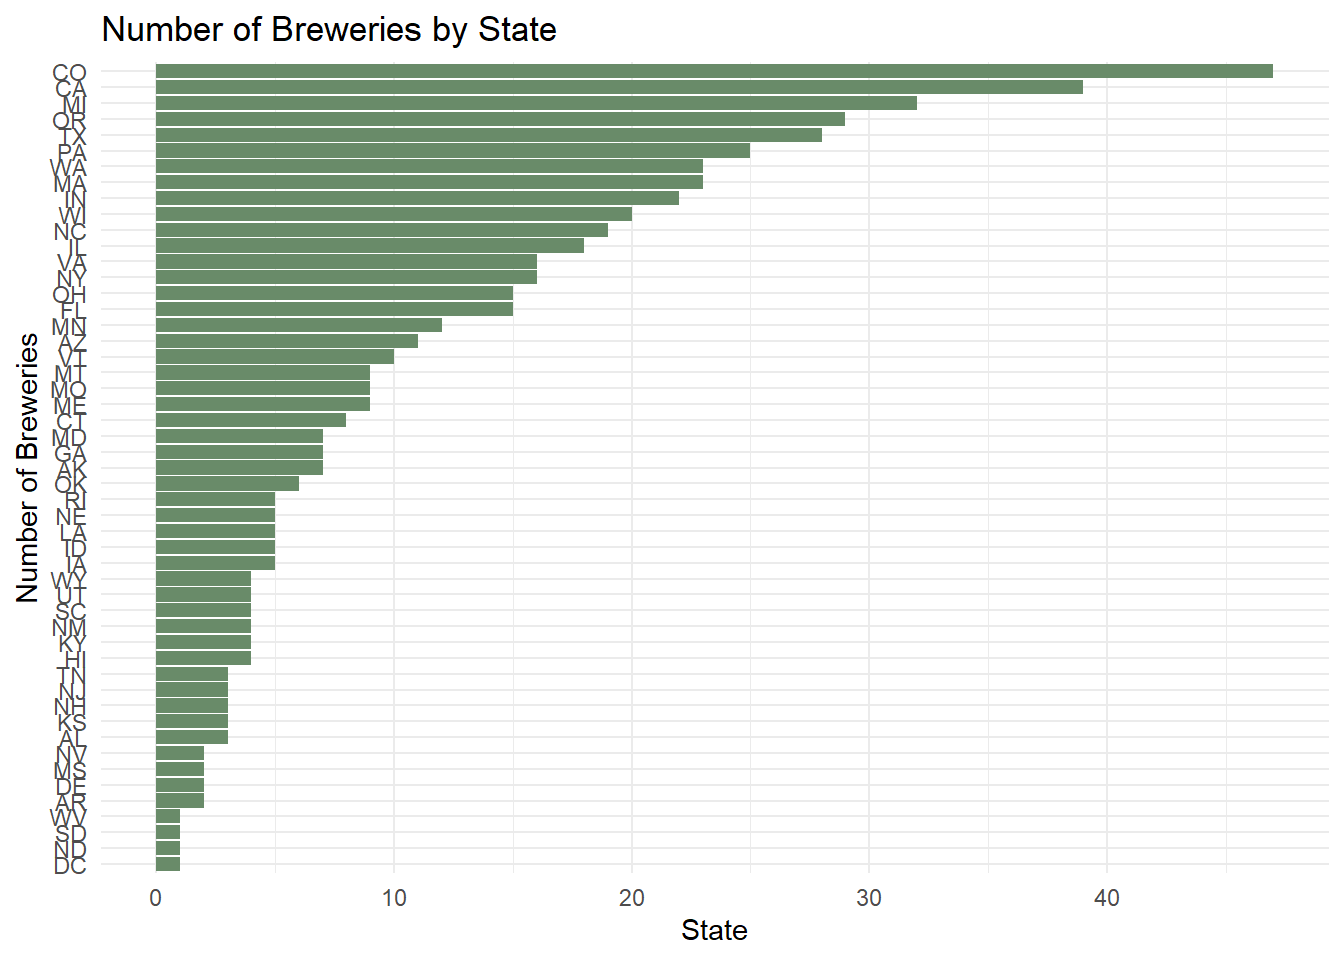
\includegraphics{Case_Study_01_files/figure-latex/State n-1.pdf}

\begin{Shaded}
\begin{Highlighting}[]
\CommentTok{\# Load in State Brewery Counts (This changes State name from "AL" {-}\textgreater{} "alabama")}
\NormalTok{states }\OtherTok{\textless{}{-}} \FunctionTok{read\_csv}\NormalTok{(}\FunctionTok{url}\NormalTok{(}\StringTok{"https://raw.githubusercontent.com/ericlaigaie/Case{-}Study{-}01/main/state\_brewery\_counts.csv"}\NormalTok{))}
\end{Highlighting}
\end{Shaded}

\begin{verbatim}
## Rows: 51 Columns: 2
\end{verbatim}

\begin{verbatim}
## -- Column specification ----------------------------------------------------------------------------
## Delimiter: ","
## chr (1): State
## dbl (1): n
\end{verbatim}

\begin{verbatim}
## 
## i Use `spec()` to retrieve the full column specification for this data.
## i Specify the column types or set `show_col_types = FALSE` to quiet this message.
\end{verbatim}

\begin{Shaded}
\begin{Highlighting}[]
\CommentTok{\# Import geojson for state polygons}
\FunctionTok{data}\NormalTok{(continental\_us\_states)}

\CommentTok{\# Designate region \& value}
\NormalTok{states}\SpecialCharTok{$}\NormalTok{region }\OtherTok{\textless{}{-}} \FunctionTok{tolower}\NormalTok{(states}\SpecialCharTok{$}\NormalTok{State)}
\NormalTok{states}\SpecialCharTok{$}\NormalTok{value }\OtherTok{\textless{}{-}}\NormalTok{ states}\SpecialCharTok{$}\NormalTok{n}

\CommentTok{\# Create Choropleth}
\FunctionTok{state\_choropleth}\NormalTok{(states, }
                 \AttributeTok{num\_colors=}\DecValTok{9}\NormalTok{,}
                 \AttributeTok{zoom =}\NormalTok{ continental\_us\_states) }\SpecialCharTok{+}
  \FunctionTok{scale\_fill\_brewer}\NormalTok{(}\AttributeTok{palette=}\StringTok{"Greens"}\NormalTok{) }\SpecialCharTok{+}
  \FunctionTok{labs}\NormalTok{(}\AttributeTok{title =} \StringTok{"Breweries by State"}\NormalTok{,}
       \AttributeTok{fill =} \StringTok{"n"}\NormalTok{) }\SpecialCharTok{+}
  \FunctionTok{guides}\NormalTok{(}\AttributeTok{fill=}\FunctionTok{guide\_legend}\NormalTok{(}\AttributeTok{title=}\StringTok{"N"}\NormalTok{))}
\end{Highlighting}
\end{Shaded}

\begin{verbatim}
## Scale for 'fill' is already present. Adding another scale for 'fill', which will replace the
## existing scale.
\end{verbatim}

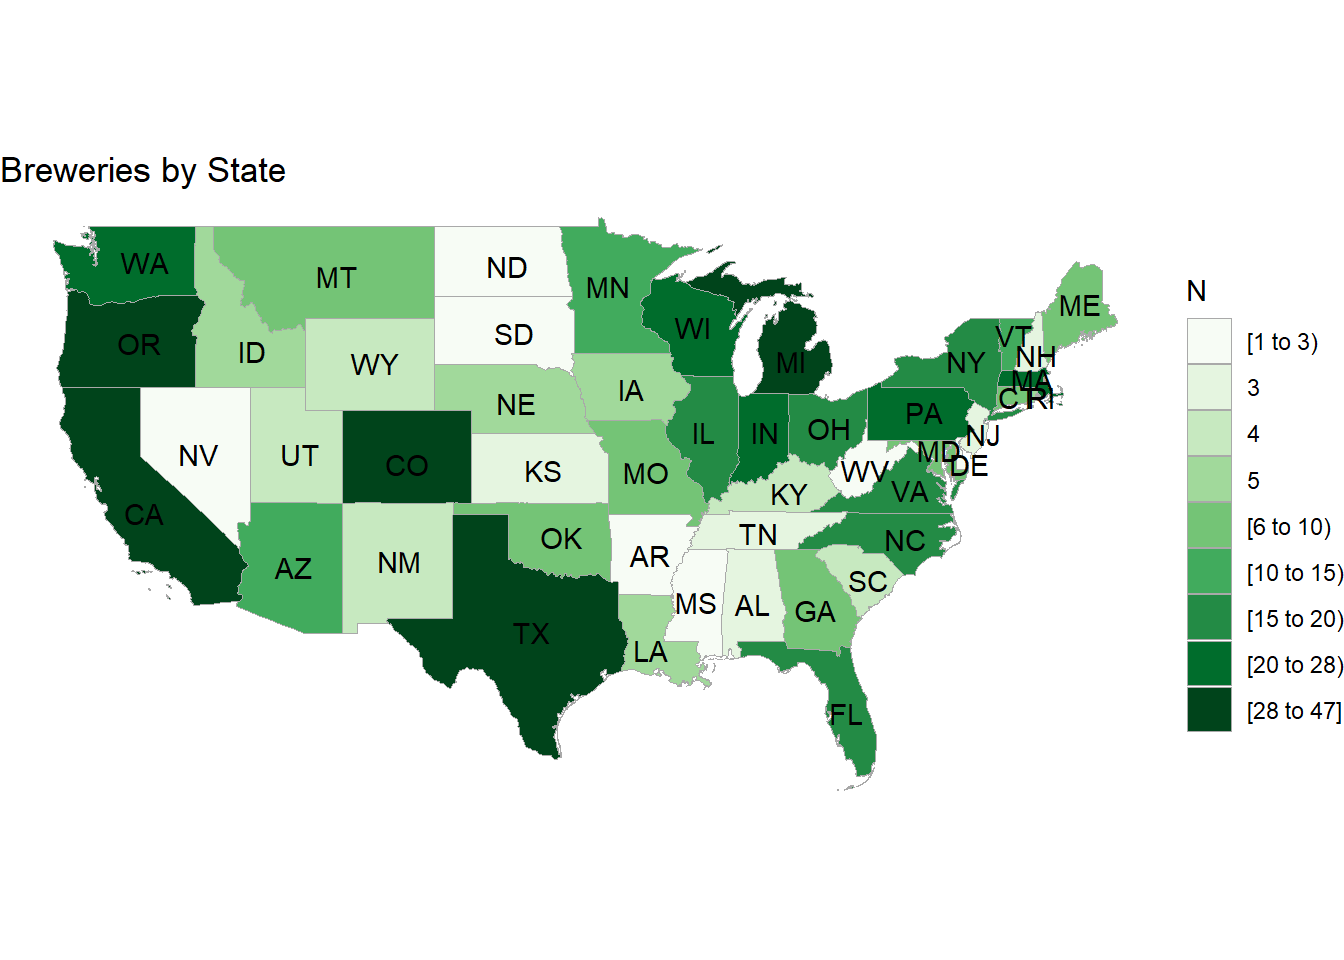
\includegraphics{Case_Study_01_files/figure-latex/State n-2.pdf} Brewery
count varies from state to state. Colorado, California, and Michigan
lead the way with over 30 breweries while the bottom 33 states have less
than 10 each. In an effort to find geographic patterns, a map was
produced. After observation, no solid conclusion was made. One
hypothesis is that coastline could increase the number of breweries, as
both coasts, Texas, and the Great Lakes region holds the majority of
breweries.

\hypertarget{merge-beer-data-with-the-breweries-data.-print-the-first-6-observations-and-the-last-six-observations-to-check-the-merged-file.-rmd-only-this-does-not-need-to-be-included-in-the-presentation-or-the-deck.}{%
\subsection{2. Merge beer data with the breweries data. Print the first
6 observations and the last six observations to check the merged file.
(RMD only, this does not need to be included in the presentation or the
deck.)}\label{merge-beer-data-with-the-breweries-data.-print-the-first-6-observations-and-the-last-six-observations-to-check-the-merged-file.-rmd-only-this-does-not-need-to-be-included-in-the-presentation-or-the-deck.}}

\begin{Shaded}
\begin{Highlighting}[]
\CommentTok{\# Merge beers and breweries}
\NormalTok{breweries }\OtherTok{\textless{}{-}}\NormalTok{ breweries }\SpecialCharTok{\%\textgreater{}\%} \FunctionTok{rename}\NormalTok{(}\AttributeTok{Brewery\_id=}\NormalTok{Brew\_ID)}
\NormalTok{df }\OtherTok{\textless{}{-}} \FunctionTok{merge}\NormalTok{(breweries, beers, }\AttributeTok{by=}\StringTok{\textquotesingle{}Brewery\_id\textquotesingle{}}\NormalTok{)}

\NormalTok{df }\OtherTok{\textless{}{-}}\NormalTok{ df }\SpecialCharTok{\%\textgreater{}\%} \FunctionTok{rename}\NormalTok{(}\AttributeTok{Brewery =}\NormalTok{ Name.x, }\AttributeTok{Beer =}\NormalTok{ Name.y)}

\CommentTok{\# Print top \& bottom 6}
\FunctionTok{head}\NormalTok{(df, }\DecValTok{6}\NormalTok{)}
\end{Highlighting}
\end{Shaded}

\begin{verbatim}
##   Brewery_id           Brewery        City State          Beer Beer_ID   ABV IBU
## 1          1 NorthGate Brewing Minneapolis    MN       Pumpion    2689 0.060  38
## 2          1 NorthGate Brewing Minneapolis    MN    Stronghold    2688 0.060  25
## 3          1 NorthGate Brewing Minneapolis    MN   Parapet ESB    2687 0.056  47
## 4          1 NorthGate Brewing Minneapolis    MN  Get Together    2692 0.045  50
## 5          1 NorthGate Brewing Minneapolis    MN Maggie's Leap    2691 0.049  26
## 6          1 NorthGate Brewing Minneapolis    MN    Wall's End    2690 0.048  19
##                                 Style Ounces
## 1                         Pumpkin Ale     16
## 2                     American Porter     16
## 3 Extra Special / Strong Bitter (ESB)     16
## 4                        American IPA     16
## 5                  Milk / Sweet Stout     16
## 6                   English Brown Ale     16
\end{verbatim}

\begin{Shaded}
\begin{Highlighting}[]
\FunctionTok{tail}\NormalTok{(df, }\DecValTok{6}\NormalTok{)}
\end{Highlighting}
\end{Shaded}

\begin{verbatim}
##      Brewery_id                       Brewery          City State                      Beer Beer_ID
## 2405        556         Ukiah Brewing Company         Ukiah    CA             Pilsner Ukiah      98
## 2406        557       Butternuts Beer and Ale Garrattsville    NY         Porkslap Pale Ale      49
## 2407        557       Butternuts Beer and Ale Garrattsville    NY           Snapperhead IPA      51
## 2408        557       Butternuts Beer and Ale Garrattsville    NY         Moo Thunder Stout      50
## 2409        557       Butternuts Beer and Ale Garrattsville    NY  Heinnieweisse Weissebier      52
## 2410        558 Sleeping Lady Brewing Company     Anchorage    AK Urban Wilderness Pale Ale      30
##        ABV IBU                   Style Ounces
## 2405 0.055  NA         German Pilsener     12
## 2406 0.043  NA American Pale Ale (APA)     12
## 2407 0.068  NA            American IPA     12
## 2408 0.049  NA      Milk / Sweet Stout     12
## 2409 0.049  NA              Hefeweizen     12
## 2410 0.049  NA        English Pale Ale     12
\end{verbatim}

After merging the datasets, we are left with a larger dataframe that not
only holds information on each brewery, but the individuals beers inside
of them.

\hypertarget{address-the-missing-values-in-each-column.}{%
\subsection{3. Address the missing values in each
column.}\label{address-the-missing-values-in-each-column.}}

\begin{Shaded}
\begin{Highlighting}[]
\CommentTok{\# METHOD 3 {-} MEAN IMPUTATION BY STYLE GROUP}

\CommentTok{\# Remove missing Styles}
\NormalTok{df }\OtherTok{\textless{}{-}}\NormalTok{ df }\SpecialCharTok{\%\textgreater{}\%} \FunctionTok{filter}\NormalTok{(}\FunctionTok{is.na}\NormalTok{(Style) }\SpecialCharTok{==} \ConstantTok{FALSE}\NormalTok{)}

\CommentTok{\# Function takes in df and imputes mean ABV and IBU. Also creates Style\_Group column}
\NormalTok{imputer }\OtherTok{\textless{}{-}} \ControlFlowTok{function}\NormalTok{(mydf, myText) \{}
\NormalTok{  temp }\OtherTok{\textless{}{-}}\NormalTok{ \{\{mydf\}\}}
  \ControlFlowTok{for}\NormalTok{(i }\ControlFlowTok{in} \DecValTok{7}\SpecialCharTok{:}\DecValTok{8}\NormalTok{)\{}
\NormalTok{    temp[}\FunctionTok{is.na}\NormalTok{(temp[,i]), i] }\OtherTok{\textless{}{-}} \FunctionTok{mean}\NormalTok{(temp[,i], }\AttributeTok{na.rm =} \ConstantTok{TRUE}\NormalTok{)}
\NormalTok{  \}}
\NormalTok{  temp}\SpecialCharTok{$}\NormalTok{Style\_Group }\OtherTok{\textless{}{-}}\NormalTok{ \{\{myText\}\}}
\NormalTok{  output }\OtherTok{\textless{}{-}}\NormalTok{ temp}
\NormalTok{\}}

\CommentTok{\# Creating new dfs for each style group}
\NormalTok{ale }\OtherTok{\textless{}{-}}\NormalTok{ df }\SpecialCharTok{\%\textgreater{}\%} \FunctionTok{filter}\NormalTok{(}\FunctionTok{grepl}\NormalTok{(}\StringTok{\textquotesingle{}Ale\textquotesingle{}}\NormalTok{, df}\SpecialCharTok{$}\NormalTok{Style) }\SpecialCharTok{==} \ConstantTok{TRUE}\NormalTok{) }\SpecialCharTok{\%\textgreater{}\%} \FunctionTok{filter}\NormalTok{(Style }\SpecialCharTok{!=} \StringTok{\textquotesingle{}English India Pale Ale (IPA)\textquotesingle{}}\NormalTok{)}
\NormalTok{ipa }\OtherTok{\textless{}{-}}\NormalTok{ df }\SpecialCharTok{\%\textgreater{}\%} \FunctionTok{filter}\NormalTok{(}\FunctionTok{grepl}\NormalTok{(}\StringTok{\textquotesingle{}IPA\textquotesingle{}}\NormalTok{, df}\SpecialCharTok{$}\NormalTok{Style) }\SpecialCharTok{==} \ConstantTok{TRUE}\NormalTok{)}
\NormalTok{lager }\OtherTok{\textless{}{-}}\NormalTok{ df }\SpecialCharTok{\%\textgreater{}\%} \FunctionTok{filter}\NormalTok{(}\FunctionTok{grepl}\NormalTok{(}\StringTok{\textquotesingle{}Lager\textquotesingle{}}\NormalTok{, df}\SpecialCharTok{$}\NormalTok{Style) }\SpecialCharTok{==} \ConstantTok{TRUE}\NormalTok{)}
\NormalTok{stout }\OtherTok{\textless{}{-}}\NormalTok{ df }\SpecialCharTok{\%\textgreater{}\%} \FunctionTok{filter}\NormalTok{(}\FunctionTok{grepl}\NormalTok{(}\StringTok{\textquotesingle{}Stout\textquotesingle{}}\NormalTok{, df}\SpecialCharTok{$}\NormalTok{Style) }\SpecialCharTok{==} \ConstantTok{TRUE}\NormalTok{)}
\NormalTok{other }\OtherTok{\textless{}{-}}\NormalTok{ df }\SpecialCharTok{\%\textgreater{}\%} \FunctionTok{filter}\NormalTok{(}\FunctionTok{grepl}\NormalTok{(}\StringTok{\textquotesingle{}Stout\textquotesingle{}}\NormalTok{, df}\SpecialCharTok{$}\NormalTok{Style) }\SpecialCharTok{==} \ConstantTok{FALSE} \SpecialCharTok{\&}
                \FunctionTok{grepl}\NormalTok{(}\StringTok{\textquotesingle{}Lager\textquotesingle{}}\NormalTok{, df}\SpecialCharTok{$}\NormalTok{Style) }\SpecialCharTok{==} \ConstantTok{FALSE} \SpecialCharTok{\&}
                \FunctionTok{grepl}\NormalTok{(}\StringTok{\textquotesingle{}IPA\textquotesingle{}}\NormalTok{, df}\SpecialCharTok{$}\NormalTok{Style) }\SpecialCharTok{==} \ConstantTok{FALSE} \SpecialCharTok{\&}
                \FunctionTok{grepl}\NormalTok{(}\StringTok{\textquotesingle{}IPA\textquotesingle{}}\NormalTok{, df}\SpecialCharTok{$}\NormalTok{Style) }\SpecialCharTok{==} \ConstantTok{FALSE} \SpecialCharTok{\&}
                \FunctionTok{grepl}\NormalTok{(}\StringTok{\textquotesingle{}Ale\textquotesingle{}}\NormalTok{, df}\SpecialCharTok{$}\NormalTok{Style) }\SpecialCharTok{==} \ConstantTok{FALSE}\NormalTok{)}

\CommentTok{\# Imputing mean ABV / IBU}
\NormalTok{ale }\OtherTok{\textless{}{-}} \FunctionTok{imputer}\NormalTok{(ale, }\StringTok{\textquotesingle{}Ale\textquotesingle{}}\NormalTok{)}
\NormalTok{ipa }\OtherTok{\textless{}{-}} \FunctionTok{imputer}\NormalTok{(ipa, }\StringTok{\textquotesingle{}IPA\textquotesingle{}}\NormalTok{)}
\NormalTok{lager }\OtherTok{\textless{}{-}} \FunctionTok{imputer}\NormalTok{(lager, }\StringTok{\textquotesingle{}Lager\textquotesingle{}}\NormalTok{)}
\NormalTok{stout }\OtherTok{\textless{}{-}} \FunctionTok{imputer}\NormalTok{(stout, }\StringTok{\textquotesingle{}Stout\textquotesingle{}}\NormalTok{)}
\NormalTok{other }\OtherTok{\textless{}{-}} \FunctionTok{imputer}\NormalTok{(other, }\StringTok{\textquotesingle{}Other\textquotesingle{}}\NormalTok{)}

\CommentTok{\# Combine back into df}
\NormalTok{df }\OtherTok{\textless{}{-}} \FunctionTok{rbind}\NormalTok{(ale, ipa, lager, stout, other)}
\NormalTok{df}\SpecialCharTok{$}\NormalTok{Style\_Group }\OtherTok{\textless{}{-}} \FunctionTok{as.factor}\NormalTok{(df}\SpecialCharTok{$}\NormalTok{Style\_Group)}
\end{Highlighting}
\end{Shaded}

Because missing values are found in over 40\% of the IBU column, it was
important to avoid removing them outright. Therefore, the dataset was
split into 5 groups based on beer style (Ale, IPA, Lager, Stout, and
Other). Then, the missing values in each group were imputed with the
group mean of that variable. Additionally, 5 missing Styles were found.
Since this missing data is a small part of the full dataframe, these
rows with missing values were removed.

\hypertarget{compute-the-median-alcohol-content-and-international-bitterness-unit-for-each-state.-plot-a-bar-chart-to-compare.}{%
\subsection{4. Compute the median alcohol content and international
bitterness unit for each state. Plot a bar chart to
compare.}\label{compute-the-median-alcohol-content-and-international-bitterness-unit-for-each-state.-plot-a-bar-chart-to-compare.}}

\begin{Shaded}
\begin{Highlighting}[]
\CommentTok{\# Median ABV bar chart}
\NormalTok{df }\SpecialCharTok{\%\textgreater{}\%} \FunctionTok{group\_by}\NormalTok{(State) }\SpecialCharTok{\%\textgreater{}\%} 
  \FunctionTok{summarise}\NormalTok{(}\AttributeTok{med\_abv =} \FunctionTok{median}\NormalTok{(ABV)) }\SpecialCharTok{\%\textgreater{}\%}
  \FunctionTok{ggplot}\NormalTok{(}\FunctionTok{aes}\NormalTok{(}\AttributeTok{y=}\FunctionTok{reorder}\NormalTok{(State, med\_abv), }\AttributeTok{x=}\NormalTok{med\_abv)) }\SpecialCharTok{+} 
  \FunctionTok{geom\_bar}\NormalTok{(}\AttributeTok{stat=}\StringTok{\textquotesingle{}identity\textquotesingle{}}\NormalTok{, }\AttributeTok{fill=}\StringTok{\textquotesingle{}darkseagreen4\textquotesingle{}}\NormalTok{) }\SpecialCharTok{+}
  \FunctionTok{labs}\NormalTok{(}\AttributeTok{x=}\StringTok{\textquotesingle{}Median ABV\textquotesingle{}}\NormalTok{, }\AttributeTok{y=}\StringTok{\textquotesingle{}State\textquotesingle{}}\NormalTok{, }\AttributeTok{title=}\StringTok{\textquotesingle{}Median ABV by State\textquotesingle{}}\NormalTok{)}
\end{Highlighting}
\end{Shaded}

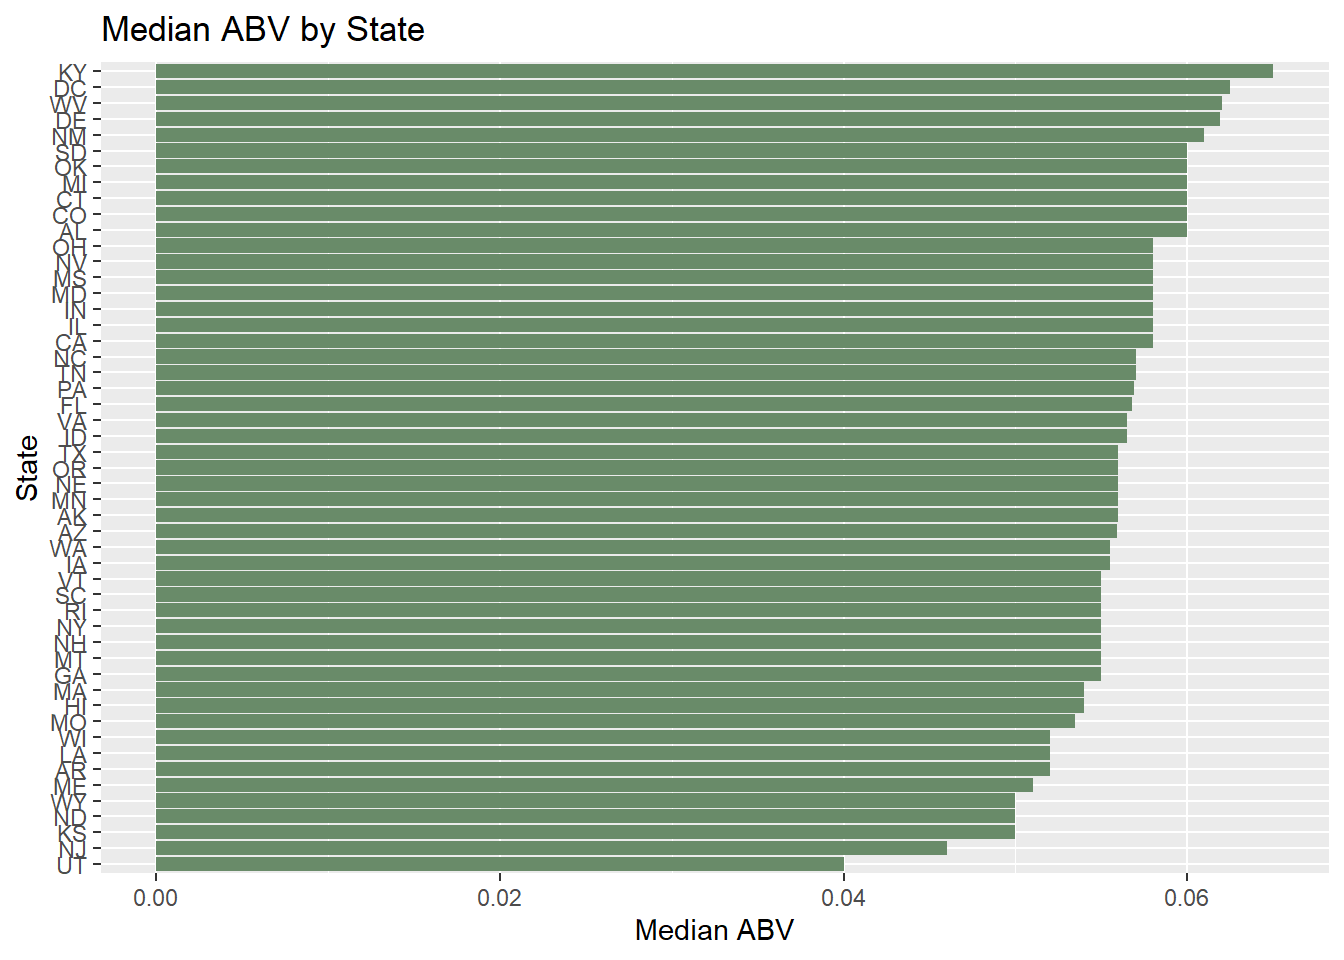
\includegraphics{Case_Study_01_files/figure-latex/med_abv-1.pdf}

\begin{Shaded}
\begin{Highlighting}[]
\CommentTok{\# Median IBU bar chart}
\NormalTok{df }\SpecialCharTok{\%\textgreater{}\%} \FunctionTok{group\_by}\NormalTok{(State) }\SpecialCharTok{\%\textgreater{}\%}
  \FunctionTok{summarise}\NormalTok{(}\AttributeTok{med\_ibu =} \FunctionTok{median}\NormalTok{(IBU)) }\SpecialCharTok{\%\textgreater{}\%}
  \FunctionTok{ggplot}\NormalTok{(}\FunctionTok{aes}\NormalTok{(}\AttributeTok{y=}\FunctionTok{reorder}\NormalTok{(State, med\_ibu), }\AttributeTok{x=}\NormalTok{med\_ibu)) }\SpecialCharTok{+} 
  \FunctionTok{geom\_bar}\NormalTok{(}\AttributeTok{stat=}\StringTok{\textquotesingle{}identity\textquotesingle{}}\NormalTok{, }\AttributeTok{fill=}\StringTok{\textquotesingle{}darkseagreen4\textquotesingle{}}\NormalTok{) }\SpecialCharTok{+}
  \FunctionTok{labs}\NormalTok{(}\AttributeTok{x=}\StringTok{\textquotesingle{}Median IBU\textquotesingle{}}\NormalTok{, }\AttributeTok{y=}\StringTok{\textquotesingle{}State\textquotesingle{}}\NormalTok{, }\AttributeTok{title=}\StringTok{\textquotesingle{}Median IBU by State\textquotesingle{}}\NormalTok{)}
\end{Highlighting}
\end{Shaded}

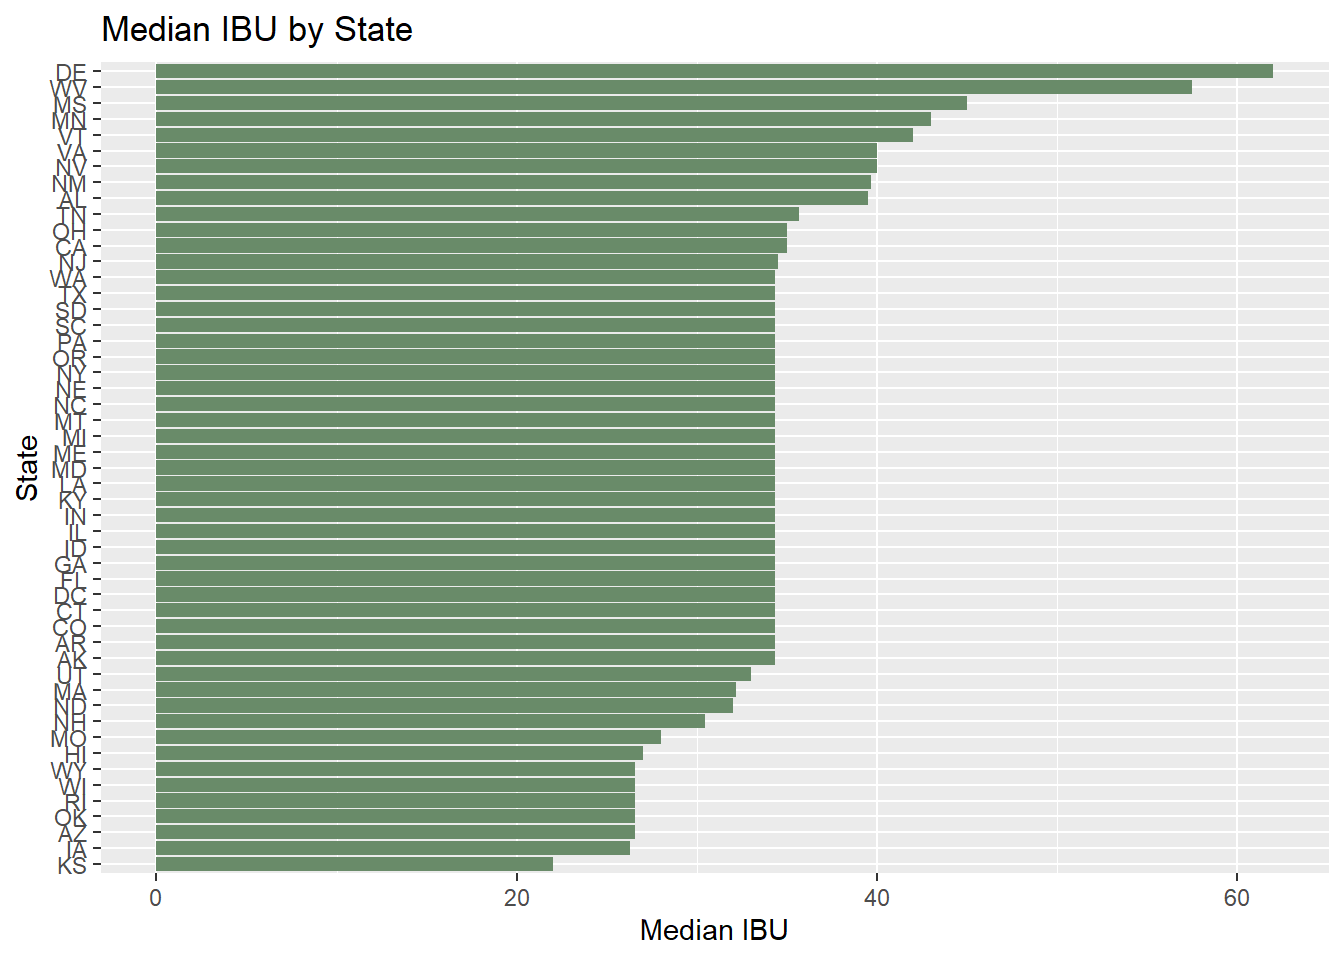
\includegraphics{Case_Study_01_files/figure-latex/med_abv-2.pdf} Both
the median ABV and IBU charts do not show a lot of variation between
states. 44/51 states have a median ABV between .05 and .06, and 40/51
states a median IBU between 30 and 50. Additionally, 25 states have an
almost identical median IBU. This is most likely a product of these
states having many missing IBU values that were imputed manually.

\hypertarget{which-state-has-the-maximum-alcoholic-abv-beer-which-state-has-the-most-bitter-ibu-beer}{%
\subsection{5. Which state has the maximum alcoholic (ABV) beer? Which
state has the most bitter (IBU)
beer?}\label{which-state-has-the-maximum-alcoholic-abv-beer-which-state-has-the-most-bitter-ibu-beer}}

\begin{Shaded}
\begin{Highlighting}[]
\CommentTok{\# Find max ABV \& IBU}
\NormalTok{max\_ABV }\OtherTok{=} \FunctionTok{max}\NormalTok{(df}\SpecialCharTok{$}\NormalTok{ABV)}
\NormalTok{max\_IBU }\OtherTok{=} \FunctionTok{max}\NormalTok{(df}\SpecialCharTok{$}\NormalTok{IBU)}
\NormalTok{df }\SpecialCharTok{\%\textgreater{}\%} \FunctionTok{filter}\NormalTok{(ABV }\SpecialCharTok{==}\NormalTok{ max\_ABV)}
\end{Highlighting}
\end{Shaded}

\begin{verbatim}
##   Brewery_id                 Brewery    City State
## 1         52 Upslope Brewing Company Boulder    CO
##                                                   Beer Beer_ID   ABV      IBU            Style
## 1 Lee Hill Series Vol. 5 - Belgian Style Quadrupel Ale    2565 0.128 26.55937 Quadrupel (Quad)
##   Ounces Style_Group
## 1   19.2       Other
\end{verbatim}

\begin{Shaded}
\begin{Highlighting}[]
\NormalTok{df }\SpecialCharTok{\%\textgreater{}\%} \FunctionTok{filter}\NormalTok{(IBU }\SpecialCharTok{==}\NormalTok{ max\_IBU)}
\end{Highlighting}
\end{Shaded}

\begin{verbatim}
##   Brewery_id                 Brewery    City State                      Beer Beer_ID   ABV IBU
## 1        375 Astoria Brewing Company Astoria    OR Bitter Bitch Imperial IPA     980 0.082 138
##                            Style Ounces Style_Group
## 1 American Double / Imperial IPA     12         IPA
\end{verbatim}

\begin{Shaded}
\begin{Highlighting}[]
\NormalTok{ABV\_diff }\OtherTok{\textless{}{-}}\NormalTok{ (max\_ABV }\SpecialCharTok{{-}} \FunctionTok{mean}\NormalTok{(df}\SpecialCharTok{$}\NormalTok{ABV)) }\SpecialCharTok{/} \FunctionTok{sd}\NormalTok{(df}\SpecialCharTok{$}\NormalTok{ABV)}
\NormalTok{IBU\_diff }\OtherTok{\textless{}{-}}\NormalTok{ (max\_IBU }\SpecialCharTok{{-}} \FunctionTok{mean}\NormalTok{(df}\SpecialCharTok{$}\NormalTok{IBU)) }\SpecialCharTok{/} \FunctionTok{sd}\NormalTok{(df}\SpecialCharTok{$}\NormalTok{IBU)}

\CommentTok{\#ABV\_diff {-}{-}{-}\textgreater{} 5.09}
\CommentTok{\#IBU\_diff {-}{-}{-}\textgreater{} 4.30}
\end{Highlighting}
\end{Shaded}

The max ABV is .128 (12.8\%), which is 5.09 standard deviations above
the mean of .06. The max IBU is 138, which is 4.30 standard deviations
above the mean of 40.97.

\hypertarget{comment-on-the-summary-statistics-and-distribution-of-the-abv-variable.}{%
\subsection{6. Comment on the summary statistics and distribution of the
ABV
variable.}\label{comment-on-the-summary-statistics-and-distribution-of-the-abv-variable.}}

\begin{Shaded}
\begin{Highlighting}[]
\CommentTok{\# Quick summary of ABV {-} full dataset}
\FunctionTok{summary}\NormalTok{(df}\SpecialCharTok{$}\NormalTok{ABV)}
\end{Highlighting}
\end{Shaded}

\begin{verbatim}
##    Min. 1st Qu.  Median    Mean 3rd Qu.    Max. 
## 0.00100 0.05000 0.05681 0.05977 0.06700 0.12800
\end{verbatim}

\begin{Shaded}
\begin{Highlighting}[]
\FunctionTok{sd}\NormalTok{(df}\SpecialCharTok{$}\NormalTok{ABV)}
\end{Highlighting}
\end{Shaded}

\begin{verbatim}
## [1] 0.01340808
\end{verbatim}

\begin{Shaded}
\begin{Highlighting}[]
\CommentTok{\# Make 4 charts}
\NormalTok{box\_all }\OtherTok{\textless{}{-}} \FunctionTok{ggplot}\NormalTok{(df, }\FunctionTok{aes}\NormalTok{(}\AttributeTok{x=}\NormalTok{ABV)) }\SpecialCharTok{+} \FunctionTok{geom\_boxplot}\NormalTok{(}\AttributeTok{fill=}\StringTok{\textquotesingle{}darkseagreen4\textquotesingle{}}\NormalTok{) }\SpecialCharTok{+} 
  \FunctionTok{labs}\NormalTok{(}\AttributeTok{x=}\StringTok{\textquotesingle{}ABV\textquotesingle{}}\NormalTok{, }\AttributeTok{title=}\StringTok{\textquotesingle{}ABV Boxplot\textquotesingle{}}\NormalTok{)}
\NormalTok{hist\_all }\OtherTok{\textless{}{-}} \FunctionTok{ggplot}\NormalTok{(df, }\FunctionTok{aes}\NormalTok{(}\AttributeTok{x=}\NormalTok{ABV)) }\SpecialCharTok{+} \FunctionTok{geom\_histogram}\NormalTok{(}\AttributeTok{binwidth =}\NormalTok{ .}\DecValTok{005}\NormalTok{, }\AttributeTok{color=}\StringTok{\textquotesingle{}black\textquotesingle{}}\NormalTok{, }\AttributeTok{fill=}\StringTok{\textquotesingle{}darkseagreen4\textquotesingle{}}\NormalTok{) }\SpecialCharTok{+}
  \FunctionTok{labs}\NormalTok{(}\AttributeTok{x=}\StringTok{\textquotesingle{}ABV\textquotesingle{}}\NormalTok{, }\AttributeTok{title=}\StringTok{\textquotesingle{}ABV Histogram\textquotesingle{}}\NormalTok{)}

\CommentTok{\# Arrange 4 charts}
\FunctionTok{ggarrange}\NormalTok{(box\_all, hist\_all, }\AttributeTok{nrow=}\DecValTok{2}\NormalTok{, }\AttributeTok{ncol=}\DecValTok{1}\NormalTok{)}
\end{Highlighting}
\end{Shaded}

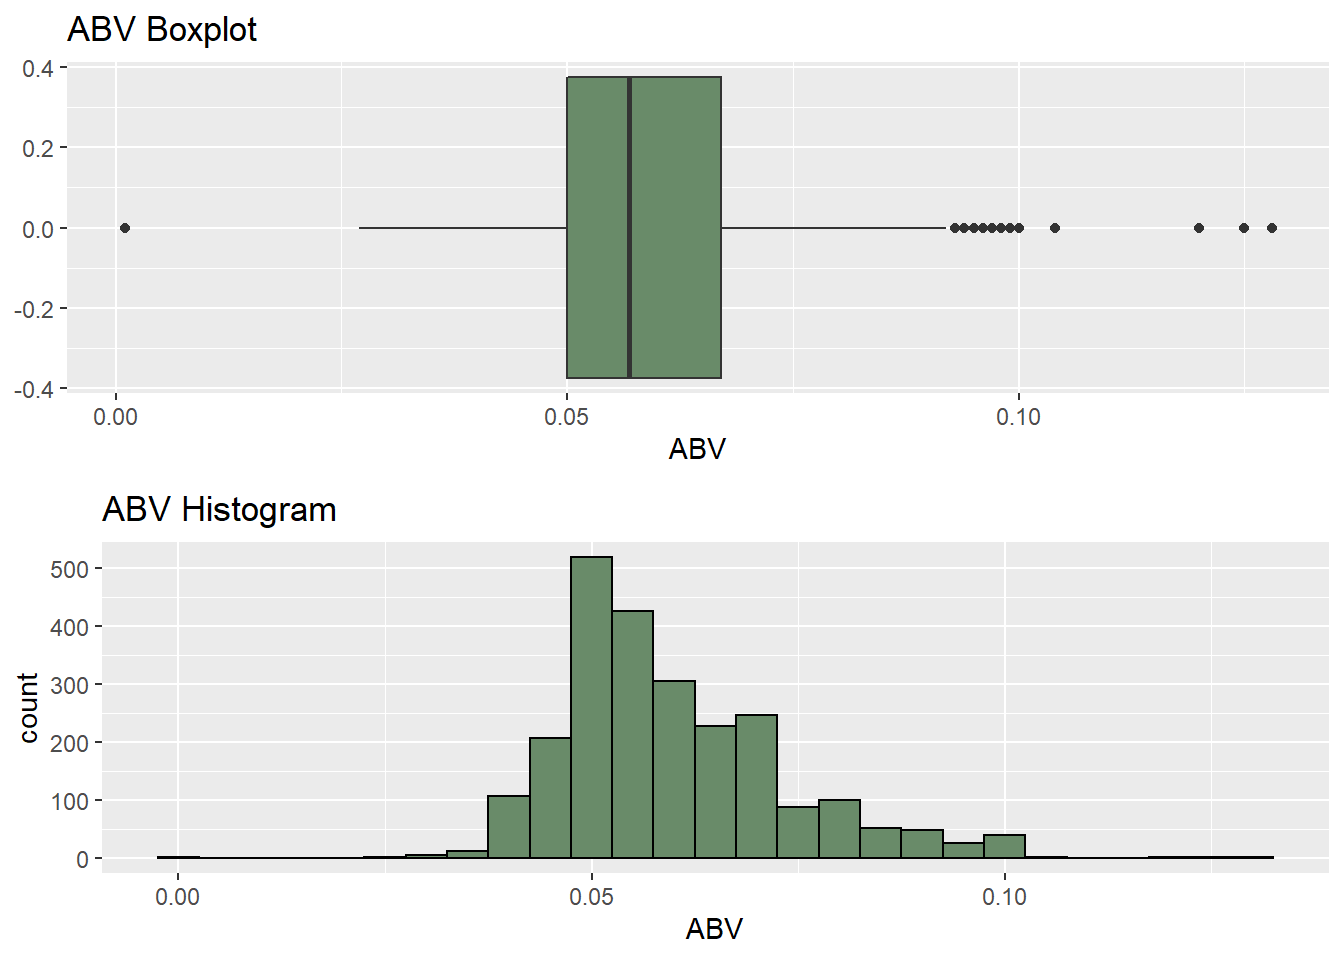
\includegraphics{Case_Study_01_files/figure-latex/unnamed-chunk-5-1.pdf}

\begin{Shaded}
\begin{Highlighting}[]
\CommentTok{\# Check for normality}
\FunctionTok{shapiro.test}\NormalTok{(df}\SpecialCharTok{$}\NormalTok{ABV)}
\end{Highlighting}
\end{Shaded}

\begin{verbatim}
## 
##  Shapiro-Wilk normality test
## 
## data:  df$ABV
## W = 0.93708, p-value < 2.2e-16
\end{verbatim}

\begin{Shaded}
\begin{Highlighting}[]
\FunctionTok{qqnorm}\NormalTok{(df}\SpecialCharTok{$}\NormalTok{ABV, }\AttributeTok{col=}\StringTok{\textquotesingle{}darkseagreen4\textquotesingle{}}\NormalTok{, }\AttributeTok{lwd=}\DecValTok{2}\NormalTok{)}
\end{Highlighting}
\end{Shaded}

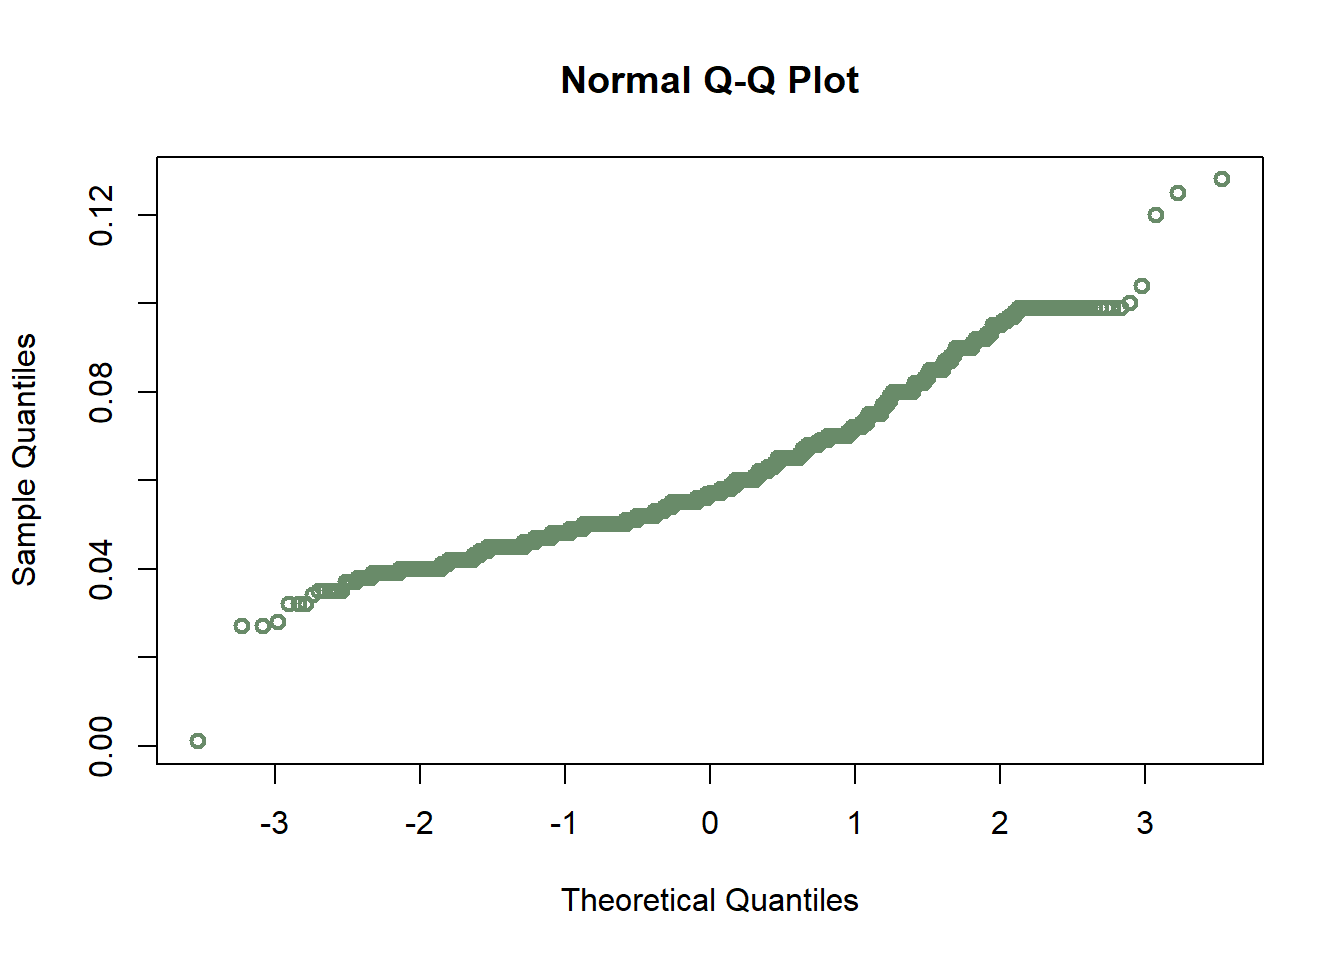
\includegraphics{Case_Study_01_files/figure-latex/unnamed-chunk-5-2.pdf}
Using both graphical and statistical methods, we concluded that the ABV
distribution is skewed right. While there is a large numbers of beers
centered around the mean of .06, there is a tail of more alcoholic beers
towards the higher ABV side.

\hypertarget{is-there-an-apparent-relationship-between-the-bitterness-of-the-beer-and-its-alcoholic-content-draw-a-scatter-plot.-make-your-best-judgment-of-a-relationship-and-explain-your-answer.}{%
\subsection{7. Is there an apparent relationship between the bitterness
of the beer and its alcoholic content? Draw a scatter plot. Make your
best judgment of a relationship and EXPLAIN your
answer.}\label{is-there-an-apparent-relationship-between-the-bitterness-of-the-beer-and-its-alcoholic-content-draw-a-scatter-plot.-make-your-best-judgment-of-a-relationship-and-explain-your-answer.}}

\begin{Shaded}
\begin{Highlighting}[]
\CommentTok{\# Find correlation of IBU and ABV in df}
\NormalTok{cor\_IBUABV }\OtherTok{=} \FunctionTok{round}\NormalTok{(}\FunctionTok{cor}\NormalTok{(df}\SpecialCharTok{$}\NormalTok{IBU, df}\SpecialCharTok{$}\NormalTok{ABV), }\DecValTok{3}\NormalTok{)}

\CommentTok{\# Make R label}
\NormalTok{label\_x }\OtherTok{=} \FunctionTok{paste}\NormalTok{(}\FunctionTok{c}\NormalTok{(}\StringTok{"R ="}\NormalTok{, cor\_IBUABV), }\AttributeTok{collapse =} \StringTok{" "}\NormalTok{)}

\CommentTok{\# IBU and ABV scatterplot (with R label)}
\FunctionTok{ggplot}\NormalTok{(df, }\FunctionTok{aes}\NormalTok{(}\AttributeTok{x=}\NormalTok{IBU, ABV)) }\SpecialCharTok{+} 
  \FunctionTok{geom\_point}\NormalTok{(}\AttributeTok{size=}\DecValTok{2}\NormalTok{, }\AttributeTok{color=}\StringTok{\textquotesingle{}darkseagreen3\textquotesingle{}}\NormalTok{) }\SpecialCharTok{+} 
  \FunctionTok{geom\_smooth}\NormalTok{(}\AttributeTok{method=}\StringTok{\textquotesingle{}lm\textquotesingle{}}\NormalTok{, }\AttributeTok{color=}\StringTok{\textquotesingle{}darkseagreen4\textquotesingle{}}\NormalTok{) }\SpecialCharTok{+}
  \FunctionTok{labs}\NormalTok{(}\AttributeTok{x=}\StringTok{\textquotesingle{}International Bittering Units (IBU)\textquotesingle{}}\NormalTok{, }\AttributeTok{y=}\StringTok{\textquotesingle{}Alcohol by Volume (ABV)\textquotesingle{}}\NormalTok{, }\AttributeTok{title=}\StringTok{\textquotesingle{}IBU vs ABV\textquotesingle{}}\NormalTok{) }\SpecialCharTok{+}
  \FunctionTok{geom\_label}\NormalTok{(}\AttributeTok{label=}\NormalTok{label\_x, }\AttributeTok{x=}\DecValTok{100}\NormalTok{, }\AttributeTok{y=}\NormalTok{.}\DecValTok{025}\NormalTok{,}\AttributeTok{label.padding =} \FunctionTok{unit}\NormalTok{(}\FloatTok{0.55}\NormalTok{, }\StringTok{"lines"}\NormalTok{), }\AttributeTok{label.size =} \FloatTok{0.35}\NormalTok{, }\AttributeTok{color =} \StringTok{"black"}\NormalTok{, }\AttributeTok{fill=}\StringTok{"\#69b3a2"}\NormalTok{)}
\end{Highlighting}
\end{Shaded}

\begin{verbatim}
## `geom_smooth()` using formula 'y ~ x'
\end{verbatim}

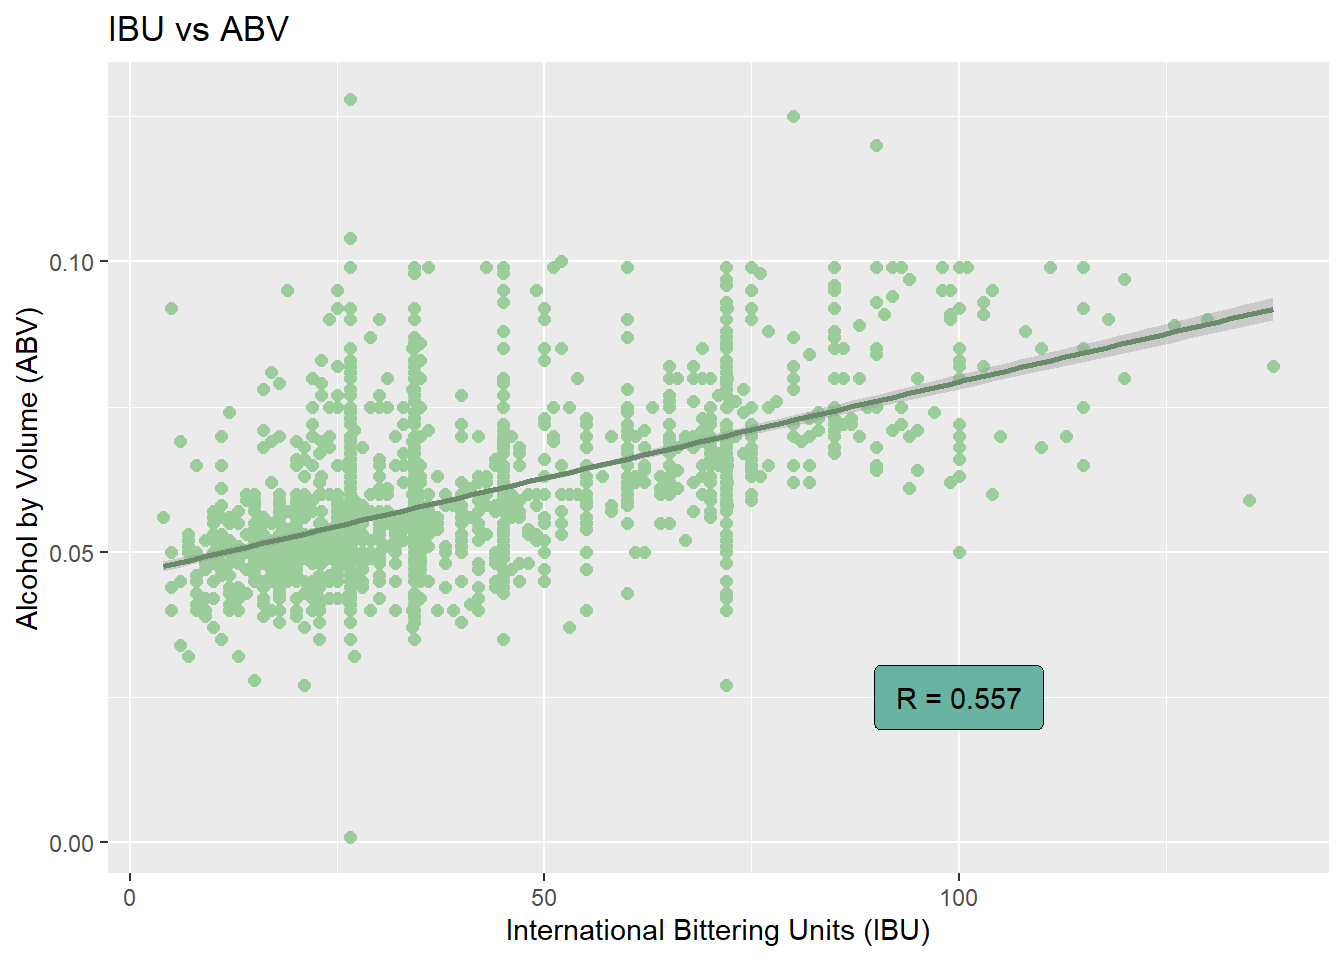
\includegraphics{Case_Study_01_files/figure-latex/unnamed-chunk-6-1.pdf}
There is a moderate positive correlation between ABV and IBU (R =
.0557). As either variable increases/decreases, we can moderately expect
the other to move in the same direction.

\hypertarget{budweiser-would-also-like-to-investigate-the-difference-with-respect-to-ibu-and-abv-between-ipas-india-pale-ales-and-other-types-of-ale-any-beer-with-ale-in-its-name-other-than-ipa.-you-decide-to-use-knn-classification-to-investigate-this-relationship.-provide-statistical-evidence-one-way-or-the-other.-you-can-of-course-assume-your-audience-is-comfortable-with-percentages-knn-is-very-easy-to-understand-conceptually.}{%
\subsection{8. Budweiser would also like to investigate the difference
with respect to IBU and ABV between IPAs (India Pale Ales) and other
types of Ale (any beer with ``Ale'' in its name other than IPA). You
decide to use KNN classification to investigate this relationship.
Provide statistical evidence one way or the other. You can of course
assume your audience is comfortable with percentages \ldots{} KNN is
very easy to understand
conceptually.}\label{budweiser-would-also-like-to-investigate-the-difference-with-respect-to-ibu-and-abv-between-ipas-india-pale-ales-and-other-types-of-ale-any-beer-with-ale-in-its-name-other-than-ipa.-you-decide-to-use-knn-classification-to-investigate-this-relationship.-provide-statistical-evidence-one-way-or-the-other.-you-can-of-course-assume-your-audience-is-comfortable-with-percentages-knn-is-very-easy-to-understand-conceptually.}}

\begin{Shaded}
\begin{Highlighting}[]
\CommentTok{\# Create new data frame with only Ale and IPA Beers}
\CommentTok{\# Next, create dummy variable for Ale vs IPA}

\NormalTok{df\_ale }\OtherTok{=}\NormalTok{ df }\SpecialCharTok{\%\textgreater{}\%} \FunctionTok{filter}\NormalTok{(}\FunctionTok{grepl}\NormalTok{(}\StringTok{"Ale"}\NormalTok{, df}\SpecialCharTok{$}\NormalTok{Style) }\SpecialCharTok{==} \ConstantTok{TRUE}\NormalTok{) }\SpecialCharTok{\%\textgreater{}\%} \FunctionTok{filter}\NormalTok{(Style }\SpecialCharTok{!=} \StringTok{\textquotesingle{}English India Pale Ale (IPA)\textquotesingle{}}\NormalTok{)}
\NormalTok{df\_IPA }\OtherTok{=}\NormalTok{ df }\SpecialCharTok{\%\textgreater{}\%} \FunctionTok{filter}\NormalTok{(}\FunctionTok{grepl}\NormalTok{(}\StringTok{"IPA"}\NormalTok{, df}\SpecialCharTok{$}\NormalTok{Style) }\SpecialCharTok{==} \ConstantTok{TRUE}\NormalTok{)}

\NormalTok{df\_IPA}\SpecialCharTok{$}\NormalTok{ale\_IPA }\OtherTok{=} \StringTok{\textquotesingle{}IPA\textquotesingle{}}
\NormalTok{df\_ale}\SpecialCharTok{$}\NormalTok{ale\_IPA }\OtherTok{=} \StringTok{\textquotesingle{}Ale\textquotesingle{}}

\NormalTok{new\_df }\OtherTok{=} \FunctionTok{rbind}\NormalTok{(df\_ale,df\_IPA)}

\NormalTok{new\_df}\SpecialCharTok{$}\NormalTok{ale\_IPA }\OtherTok{=} \FunctionTok{as.factor}\NormalTok{(new\_df}\SpecialCharTok{$}\NormalTok{ale\_IPA)}

\NormalTok{new\_df }\OtherTok{\textless{}{-}}\NormalTok{ df }\SpecialCharTok{\%\textgreater{}\%} \FunctionTok{filter}\NormalTok{(Style\_Group }\SpecialCharTok{\%in\%} \FunctionTok{c}\NormalTok{(}\StringTok{\textquotesingle{}Ale\textquotesingle{}}\NormalTok{, }\StringTok{\textquotesingle{}IPA\textquotesingle{}}\NormalTok{))}

\CommentTok{\# Perform KNN model using ABV and IBU}
\CommentTok{\# Hyper{-}tune to be completed on K value}

\CommentTok{\# First, standardize IBU and ABV values}

\NormalTok{new\_df}\SpecialCharTok{$}\NormalTok{zABV }\OtherTok{=} \FunctionTok{as.numeric}\NormalTok{(}\FunctionTok{scale}\NormalTok{(new\_df}\SpecialCharTok{$}\NormalTok{ABV))}
\NormalTok{new\_df}\SpecialCharTok{$}\NormalTok{zIBU }\OtherTok{=} \FunctionTok{as.numeric}\NormalTok{(}\FunctionTok{scale}\NormalTok{(new\_df}\SpecialCharTok{$}\NormalTok{IBU))}

\CommentTok{\# Loop to find best value for K with 70/30 train{-}test split}

\NormalTok{iterations }\OtherTok{=} \DecValTok{100}
\NormalTok{numks }\OtherTok{=} \DecValTok{100}
\NormalTok{splitPerc }\OtherTok{=}\NormalTok{ .}\DecValTok{70}

\NormalTok{masterAcc }\OtherTok{=} \FunctionTok{matrix}\NormalTok{(}\AttributeTok{nrow =}\NormalTok{ iterations, }\AttributeTok{ncol =}\NormalTok{ numks)}
\NormalTok{masterSen }\OtherTok{=} \FunctionTok{matrix}\NormalTok{(}\AttributeTok{nrow =}\NormalTok{ iterations, }\AttributeTok{ncol =}\NormalTok{ numks)}
\NormalTok{masterSpe }\OtherTok{=} \FunctionTok{matrix}\NormalTok{(}\AttributeTok{nrow =}\NormalTok{ iterations, }\AttributeTok{ncol =}\NormalTok{ numks)}

\ControlFlowTok{for}\NormalTok{(j }\ControlFlowTok{in} \DecValTok{1}\SpecialCharTok{:}\NormalTok{iterations)}
\NormalTok{\{}
\NormalTok{  trainIndices }\OtherTok{=} \FunctionTok{sample}\NormalTok{(}\DecValTok{1}\SpecialCharTok{:}\FunctionTok{dim}\NormalTok{(new\_df)[}\DecValTok{1}\NormalTok{],}\FunctionTok{round}\NormalTok{(splitPerc }\SpecialCharTok{*} \FunctionTok{dim}\NormalTok{(new\_df)[}\DecValTok{1}\NormalTok{]))}
\NormalTok{  train }\OtherTok{=}\NormalTok{ new\_df[trainIndices,]}
\NormalTok{  test }\OtherTok{=}\NormalTok{ new\_df[}\SpecialCharTok{{-}}\NormalTok{trainIndices,]}
  \ControlFlowTok{for}\NormalTok{(i }\ControlFlowTok{in} \DecValTok{1}\SpecialCharTok{:}\NormalTok{numks)}
\NormalTok{  \{}
\NormalTok{    classifications }\OtherTok{=} \FunctionTok{knn}\NormalTok{(train[,}\FunctionTok{c}\NormalTok{(}\DecValTok{7}\NormalTok{,}\DecValTok{8}\NormalTok{)],test[,}\FunctionTok{c}\NormalTok{(}\DecValTok{7}\NormalTok{,}\DecValTok{8}\NormalTok{)],train}\SpecialCharTok{$}\NormalTok{Style\_Group, }\AttributeTok{prob =} \ConstantTok{TRUE}\NormalTok{, }\AttributeTok{k =}\NormalTok{ i)}
    \FunctionTok{table}\NormalTok{(classifications,test}\SpecialCharTok{$}\NormalTok{Style\_Group)}
\NormalTok{    CM }\OtherTok{=} \FunctionTok{confusionMatrix}\NormalTok{(}\FunctionTok{table}\NormalTok{(classifications,test}\SpecialCharTok{$}\NormalTok{Style\_Group))}
\NormalTok{    masterAcc[j,i] }\OtherTok{=}\NormalTok{ CM}\SpecialCharTok{$}\NormalTok{overall[}\DecValTok{1}\NormalTok{]}
\NormalTok{    masterSen[j,i] }\OtherTok{=}\NormalTok{ CM}\SpecialCharTok{$}\NormalTok{byClass[}\DecValTok{1}\NormalTok{]}
\NormalTok{    masterSpe[j,i] }\OtherTok{=}\NormalTok{ CM}\SpecialCharTok{$}\NormalTok{byClass[}\DecValTok{2}\NormalTok{]}
\NormalTok{  \}}
  
\NormalTok{\}}

\NormalTok{MeanAcc }\OtherTok{=} \FunctionTok{colMeans}\NormalTok{(masterAcc)}
\NormalTok{MeanSen }\OtherTok{=} \FunctionTok{colMeans}\NormalTok{(masterSen)}
\NormalTok{MeanSpe }\OtherTok{=} \FunctionTok{colMeans}\NormalTok{(masterSpe)}

\FunctionTok{plot}\NormalTok{(}\FunctionTok{seq}\NormalTok{(}\DecValTok{1}\NormalTok{,numks,}\DecValTok{1}\NormalTok{),MeanAcc, }\AttributeTok{type =} \StringTok{"l"}\NormalTok{)}
\end{Highlighting}
\end{Shaded}

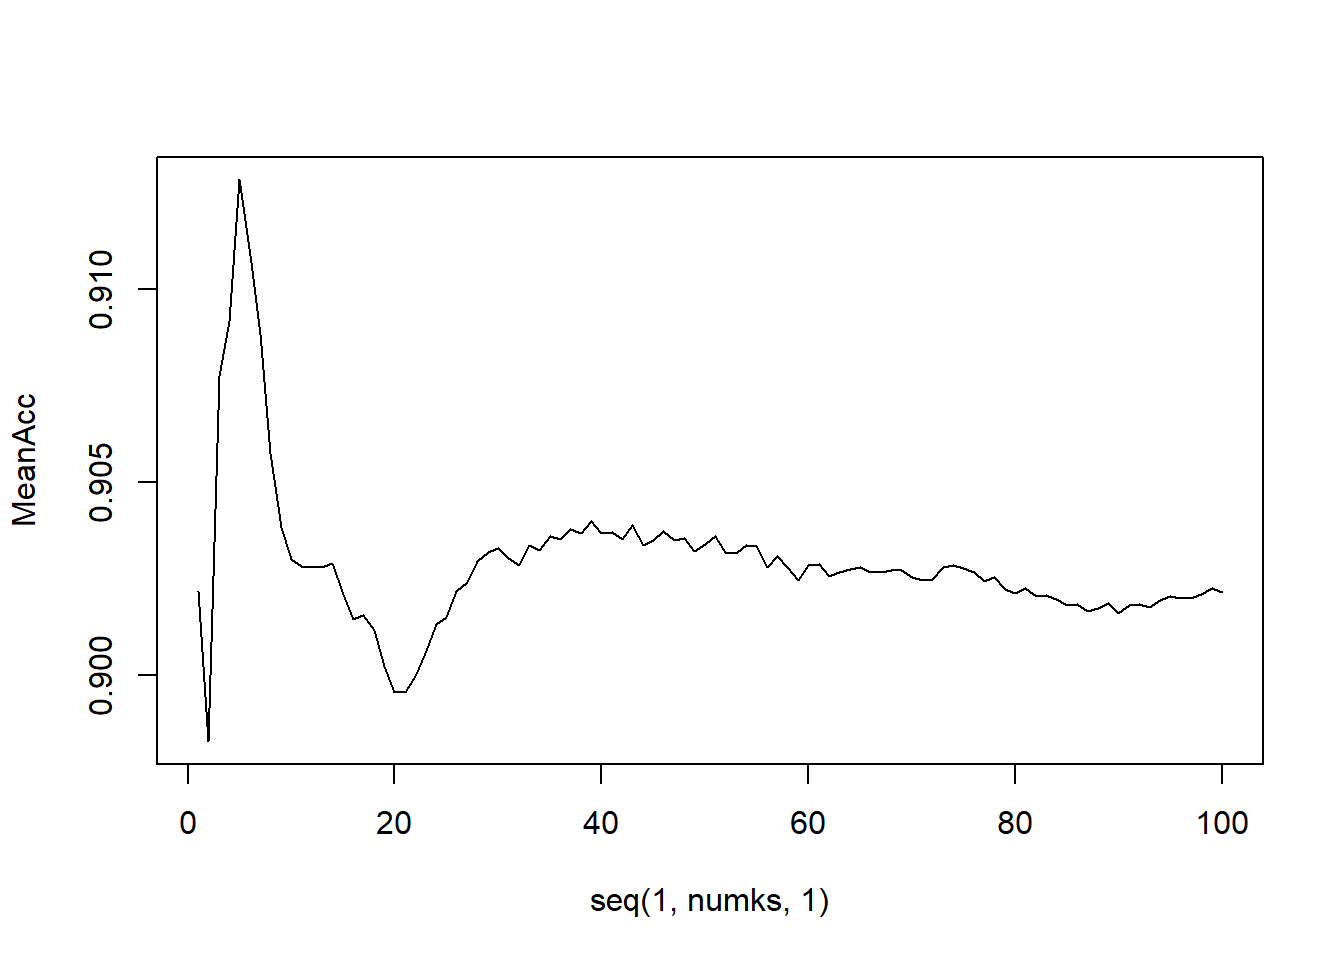
\includegraphics{Case_Study_01_files/figure-latex/unnamed-chunk-7-1.pdf}

\begin{Shaded}
\begin{Highlighting}[]
\FunctionTok{which.max}\NormalTok{(MeanAcc)}
\end{Highlighting}
\end{Shaded}

\begin{verbatim}
## [1] 5
\end{verbatim}

\begin{Shaded}
\begin{Highlighting}[]
\FunctionTok{max}\NormalTok{(MeanAcc)}
\end{Highlighting}
\end{Shaded}

\begin{verbatim}
## [1] 0.9124783
\end{verbatim}

\begin{Shaded}
\begin{Highlighting}[]
\FunctionTok{plot}\NormalTok{(}\FunctionTok{seq}\NormalTok{(}\DecValTok{1}\NormalTok{,numks,}\DecValTok{1}\NormalTok{),MeanSen, }\AttributeTok{type =} \StringTok{"l"}\NormalTok{)}
\end{Highlighting}
\end{Shaded}

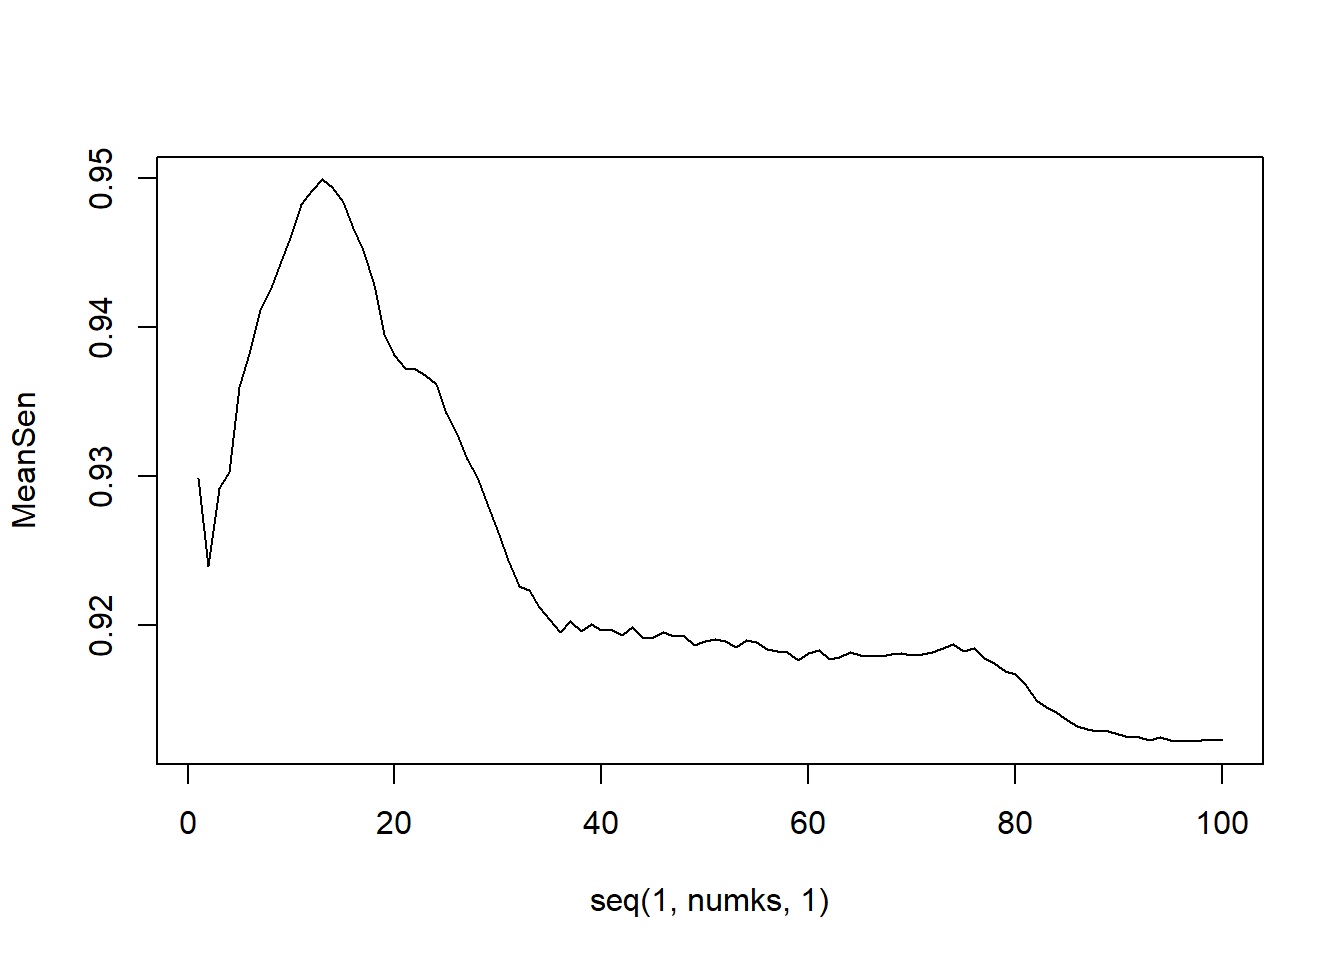
\includegraphics{Case_Study_01_files/figure-latex/unnamed-chunk-7-2.pdf}

\begin{Shaded}
\begin{Highlighting}[]
\FunctionTok{which.max}\NormalTok{(MeanSen)}
\end{Highlighting}
\end{Shaded}

\begin{verbatim}
## [1] 13
\end{verbatim}

\begin{Shaded}
\begin{Highlighting}[]
\FunctionTok{max}\NormalTok{(MeanSen)}
\end{Highlighting}
\end{Shaded}

\begin{verbatim}
## [1] 0.9463244
\end{verbatim}

\begin{Shaded}
\begin{Highlighting}[]
\FunctionTok{plot}\NormalTok{(}\FunctionTok{seq}\NormalTok{(}\DecValTok{1}\NormalTok{,numks,}\DecValTok{1}\NormalTok{),MeanSpe, }\AttributeTok{type =} \StringTok{"l"}\NormalTok{)}
\end{Highlighting}
\end{Shaded}

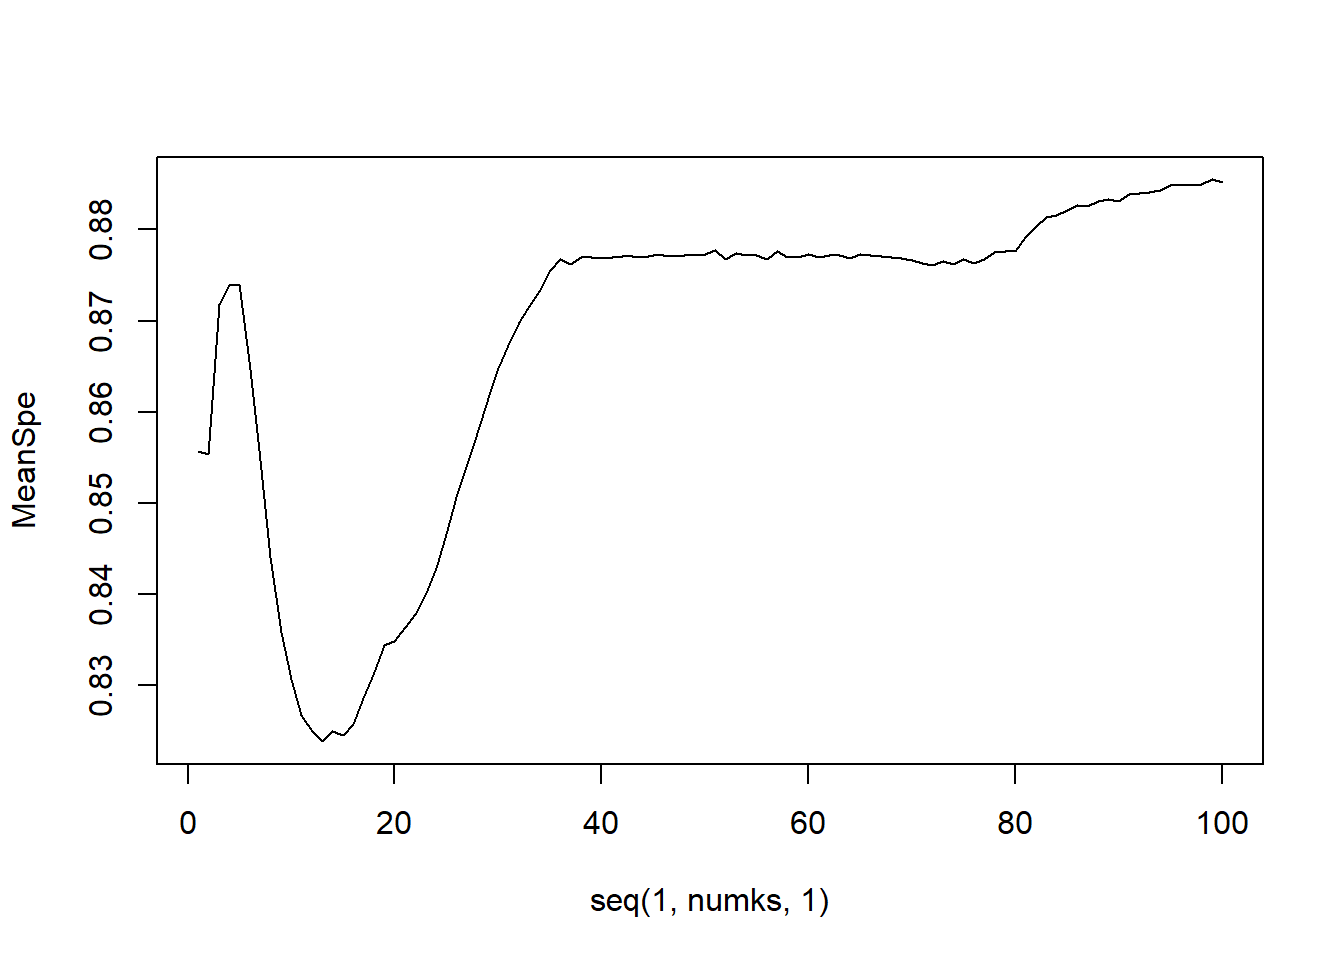
\includegraphics{Case_Study_01_files/figure-latex/unnamed-chunk-7-3.pdf}

\begin{Shaded}
\begin{Highlighting}[]
\FunctionTok{which.max}\NormalTok{(MeanSpe)}
\end{Highlighting}
\end{Shaded}

\begin{verbatim}
## [1] 97
\end{verbatim}

\begin{Shaded}
\begin{Highlighting}[]
\FunctionTok{max}\NormalTok{(MeanSpe)}
\end{Highlighting}
\end{Shaded}

\begin{verbatim}
## [1] 0.8847667
\end{verbatim}

\begin{Shaded}
\begin{Highlighting}[]
\CommentTok{\# K = 6 gives highest accuracy (81\%)}
\CommentTok{\# K = 10 gives highest sensitivity (87\%)}
\CommentTok{\# K = 62 gives highest specificity (73\%)}

\CommentTok{\# Run KNN model with K=6 for highest accuracy (per hyper tuning)}
\NormalTok{classifications }\OtherTok{=} \FunctionTok{knn}\NormalTok{(train[,}\FunctionTok{c}\NormalTok{(}\DecValTok{7}\NormalTok{,}\DecValTok{8}\NormalTok{)],test[,}\FunctionTok{c}\NormalTok{(}\DecValTok{7}\NormalTok{,}\DecValTok{8}\NormalTok{)],train}\SpecialCharTok{$}\NormalTok{Style\_Group,}\AttributeTok{prob =} \ConstantTok{TRUE}\NormalTok{, }\AttributeTok{k =} \DecValTok{5}\NormalTok{)}
\FunctionTok{confusionMatrix}\NormalTok{(}\FunctionTok{table}\NormalTok{(classifications,test}\SpecialCharTok{$}\NormalTok{Style\_Group))}
\end{Highlighting}
\end{Shaded}

\begin{verbatim}
## Confusion Matrix and Statistics
## 
##                
## classifications Ale IPA Lager Other Stout
##           Ale   272  19     0     0     0
##           IPA    21 148     0     0     0
##           Lager   0   0     0     0     0
##           Other   0   0     0     0     0
##           Stout   0   0     0     0     0
## 
## Overall Statistics
##                                           
##                Accuracy : 0.913           
##                  95% CI : (0.8835, 0.9372)
##     No Information Rate : 0.637           
##     P-Value [Acc > NIR] : < 2.2e-16       
##                                           
##                   Kappa : 0.8125          
##                                           
##  Mcnemar's Test P-Value : NA              
## 
## Statistics by Class:
## 
##                      Class: Ale Class: IPA Class: Lager Class: Other Class: Stout
## Sensitivity              0.9283     0.8862           NA           NA           NA
## Specificity              0.8862     0.9283            1            1            1
## Pos Pred Value           0.9347     0.8757           NA           NA           NA
## Neg Pred Value           0.8757     0.9347           NA           NA           NA
## Prevalence               0.6370     0.3630            0            0            0
## Detection Rate           0.5913     0.3217            0            0            0
## Detection Prevalence     0.6326     0.3674            0            0            0
## Balanced Accuracy        0.9073     0.9073           NA           NA           NA
\end{verbatim}

A KNN model using k=5 was found to produce the highest average accuracy
at 91.3\%. Therefore, an optimized KNN model could accurately predict
\textgreater90\% of beers as Ales or IPAs based solely on their ABV and
IBU. This tells us that ABV and IBU is homogenous within the Ale or IPA
style or sub-styles. Basically, if a beer with X ABV and Y IBU is an
Ale, it is likely that the majority of the most similar beers are Ales
as well.

\hypertarget{additional-modeling}{%
\subsection{8.5: Additional Modeling}\label{additional-modeling}}

In addition, while you have decided to use KNN to investigate this
relationship (KNN is required) you may also feel free to supplement your
response to this question with any other methods or techniques you have
learned. Creativity and alternative solutions are always encouraged.

\begin{Shaded}
\begin{Highlighting}[]
\CommentTok{\# Using Naive{-}Bayes to investigate relationship}

\CommentTok{\# Set seed and create Train/Test Split }
\FunctionTok{set.seed}\NormalTok{(}\DecValTok{10}\NormalTok{)}
\NormalTok{trainIndices }\OtherTok{=} \FunctionTok{sample}\NormalTok{(}\FunctionTok{seq}\NormalTok{(}\DecValTok{1}\SpecialCharTok{:}\FunctionTok{length}\NormalTok{(new\_df}\SpecialCharTok{$}\NormalTok{Beer\_ID)),}\FunctionTok{round}\NormalTok{(.}\DecValTok{7}\SpecialCharTok{*}\FunctionTok{length}\NormalTok{(new\_df}\SpecialCharTok{$}\NormalTok{Beer\_ID)))}
\NormalTok{train\_nb }\OtherTok{=}\NormalTok{ new\_df[trainIndices,]}
\NormalTok{test\_nb }\OtherTok{=}\NormalTok{ new\_df[}\SpecialCharTok{{-}}\NormalTok{trainIndices,]}

\CommentTok{\# Create model and print confusion matrix}
\NormalTok{model }\OtherTok{=} \FunctionTok{naiveBayes}\NormalTok{(train\_nb[,}\FunctionTok{c}\NormalTok{(}\DecValTok{7}\NormalTok{,}\DecValTok{8}\NormalTok{)],train\_nb}\SpecialCharTok{$}\NormalTok{Style\_Group,}\AttributeTok{laplace =} \DecValTok{1}\NormalTok{)}
\FunctionTok{table}\NormalTok{(}\FunctionTok{predict}\NormalTok{(model,test\_nb[,}\FunctionTok{c}\NormalTok{(}\DecValTok{7}\NormalTok{,}\DecValTok{8}\NormalTok{)]),test\_nb}\SpecialCharTok{$}\NormalTok{Style\_Group)}
\end{Highlighting}
\end{Shaded}

\begin{verbatim}
##        
##         Ale IPA Lager Other Stout
##   Ale   269  22     0     0     0
##   IPA    20 149     0     0     0
##   Lager   0   0     0     0     0
##   Other   0   0     0     0     0
##   Stout   0   0     0     0     0
\end{verbatim}

\begin{Shaded}
\begin{Highlighting}[]
\NormalTok{CM }\OtherTok{=} \FunctionTok{confusionMatrix}\NormalTok{(}\FunctionTok{table}\NormalTok{(}\FunctionTok{predict}\NormalTok{(model,test\_nb[,}\FunctionTok{c}\NormalTok{(}\DecValTok{7}\NormalTok{,}\DecValTok{8}\NormalTok{)]),test\_nb}\SpecialCharTok{$}\NormalTok{Style\_Group))}
\NormalTok{CM}
\end{Highlighting}
\end{Shaded}

\begin{verbatim}
## Confusion Matrix and Statistics
## 
##        
##         Ale IPA Lager Other Stout
##   Ale   269  22     0     0     0
##   IPA    20 149     0     0     0
##   Lager   0   0     0     0     0
##   Other   0   0     0     0     0
##   Stout   0   0     0     0     0
## 
## Overall Statistics
##                                           
##                Accuracy : 0.9087          
##                  95% CI : (0.8786, 0.9334)
##     No Information Rate : 0.6283          
##     P-Value [Acc > NIR] : < 2.2e-16       
##                                           
##                   Kappa : 0.8041          
##                                           
##  Mcnemar's Test P-Value : NA              
## 
## Statistics by Class:
## 
##                      Class: Ale Class: IPA Class: Lager Class: Other Class: Stout
## Sensitivity              0.9308     0.8713           NA           NA           NA
## Specificity              0.8713     0.9308            1            1            1
## Pos Pred Value           0.9244     0.8817           NA           NA           NA
## Neg Pred Value           0.8817     0.9244           NA           NA           NA
## Prevalence               0.6283     0.3717            0            0            0
## Detection Rate           0.5848     0.3239            0            0            0
## Detection Prevalence     0.6326     0.3674            0            0            0
## Balanced Accuracy        0.9011     0.9011           NA           NA           NA
\end{verbatim}

A Naive-Bayes model has similar results to our optimized KNN. This model
has a \textgreater90\% accuracy rate, meaning that it can predict
correctly if a beer is an Ale or IPA with only the ABV and IBU (and some
probability calculations).

\hypertarget{knock-their-socks-off-find-one-other-useful-inference-from-the-data-that-you-feel-budweiser-may-be-able-to-find-value-in.-you-must-convince-them-why-it-is-important-and-back-up-your-conviction-with-appropriate-statistical-evidence.}{%
\subsection{9. Knock their socks off! Find one other useful inference
from the data that you feel Budweiser may be able to find value in. You
must convince them why it is important and back up your conviction with
appropriate statistical
evidence.}\label{knock-their-socks-off-find-one-other-useful-inference-from-the-data-that-you-feel-budweiser-may-be-able-to-find-value-in.-you-must-convince-them-why-it-is-important-and-back-up-your-conviction-with-appropriate-statistical-evidence.}}

\hypertarget{load-in-regions-data-and-visualize.}{%
\subsubsection{Load in Regions data and
visualize.}\label{load-in-regions-data-and-visualize.}}

\begin{Shaded}
\begin{Highlighting}[]
\CommentTok{\# Load in regions data}
\NormalTok{regions }\OtherTok{=} \FunctionTok{read\_csv}\NormalTok{(}\FunctionTok{url}\NormalTok{(}\StringTok{\textquotesingle{}https://raw.githubusercontent.com/ericlaigaie/Case{-}Study{-}01/main/regions\_v2.csv\textquotesingle{}}\NormalTok{))}
\end{Highlighting}
\end{Shaded}

\begin{verbatim}
## Rows: 51 Columns: 3
\end{verbatim}

\begin{verbatim}
## -- Column specification ----------------------------------------------------------------------------
## Delimiter: ","
## chr (3): State, Region, State Abbreviation
\end{verbatim}

\begin{verbatim}
## 
## i Use `spec()` to retrieve the full column specification for this data.
## i Specify the column types or set `show_col_types = FALSE` to quiet this message.
\end{verbatim}

\begin{Shaded}
\begin{Highlighting}[]
\CommentTok{\# remove State Column and rename abbreviations to \textquotesingle{}State\textquotesingle{} to merge}
\NormalTok{regions }\OtherTok{=} \FunctionTok{subset}\NormalTok{(regions, }\AttributeTok{select =} \SpecialCharTok{{-}}\FunctionTok{c}\NormalTok{(State))}
\FunctionTok{names}\NormalTok{(regions)[}\DecValTok{2}\NormalTok{] }\OtherTok{=} \StringTok{\textquotesingle{}State\textquotesingle{}}
\NormalTok{df }\OtherTok{=} \FunctionTok{merge}\NormalTok{(df,regions,}\StringTok{"State"}\NormalTok{)}

\CommentTok{\# Prep data for choropleth}
\NormalTok{df}\SpecialCharTok{$}\NormalTok{Region }\OtherTok{\textless{}{-}} \FunctionTok{as.factor}\NormalTok{(df}\SpecialCharTok{$}\NormalTok{Region)}
\NormalTok{regions }\OtherTok{\textless{}{-}}\NormalTok{ regions }\SpecialCharTok{\%\textgreater{}\%} \FunctionTok{arrange}\NormalTok{(State)}

\CommentTok{\# Designate region \& value}
\NormalTok{choro\_df }\OtherTok{\textless{}{-}} \FunctionTok{data.frame}\NormalTok{(}\StringTok{\textquotesingle{}region\textquotesingle{}} \OtherTok{=}\NormalTok{ states}\SpecialCharTok{$}\NormalTok{State, }\StringTok{\textquotesingle{}value\textquotesingle{}} \OtherTok{=}\NormalTok{ regions}\SpecialCharTok{$}\NormalTok{Region)}

\CommentTok{\# Create Choropleth}
\FunctionTok{state\_choropleth}\NormalTok{(choro\_df, }
                 \AttributeTok{num\_colors=}\DecValTok{7}\NormalTok{,}
                 \AttributeTok{zoom =}\NormalTok{ continental\_us\_states) }\SpecialCharTok{+}
  \FunctionTok{scale\_fill\_brewer}\NormalTok{(}\AttributeTok{palette=}\StringTok{"Set1"}\NormalTok{) }\SpecialCharTok{+}
  \FunctionTok{labs}\NormalTok{(}\AttributeTok{title =} \StringTok{"Regions"}\NormalTok{,}
       \AttributeTok{fill =} \StringTok{"n"}\NormalTok{) }\SpecialCharTok{+}
  \FunctionTok{guides}\NormalTok{(}\AttributeTok{fill=}\FunctionTok{guide\_legend}\NormalTok{(}\AttributeTok{title=}\StringTok{"Region"}\NormalTok{))}
\end{Highlighting}
\end{Shaded}

\begin{verbatim}
## Scale for 'fill' is already present. Adding another scale for 'fill', which will replace the
## existing scale.
\end{verbatim}

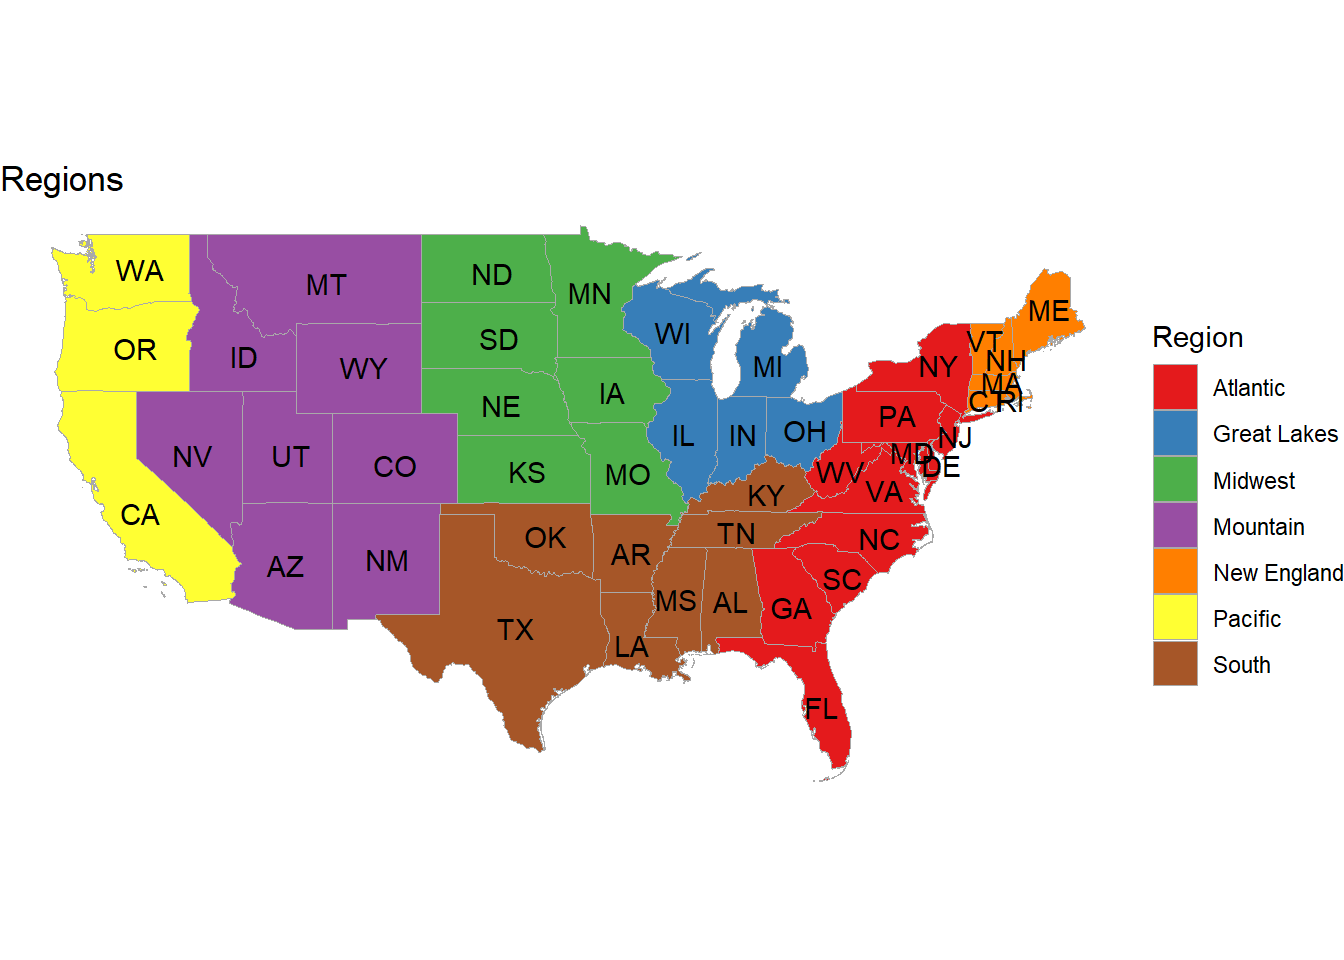
\includegraphics{Case_Study_01_files/figure-latex/unnamed-chunk-9-1.pdf}
This is a map of our regions. The next code cell will use statistical
tests to examine how ABV and IBU distributions differ between regions.

\hypertarget{checking-assumptions-of-anova}{%
\subsubsection{Checking Assumptions of
ANOVA}\label{checking-assumptions-of-anova}}

\begin{Shaded}
\begin{Highlighting}[]
\CommentTok{\# ABV}
\FunctionTok{ggplot}\NormalTok{(df, }\FunctionTok{aes}\NormalTok{(}\AttributeTok{x=}\NormalTok{ABV, }\AttributeTok{y=}\NormalTok{Region)) }\SpecialCharTok{+} \FunctionTok{geom\_boxplot}\NormalTok{()}
\end{Highlighting}
\end{Shaded}

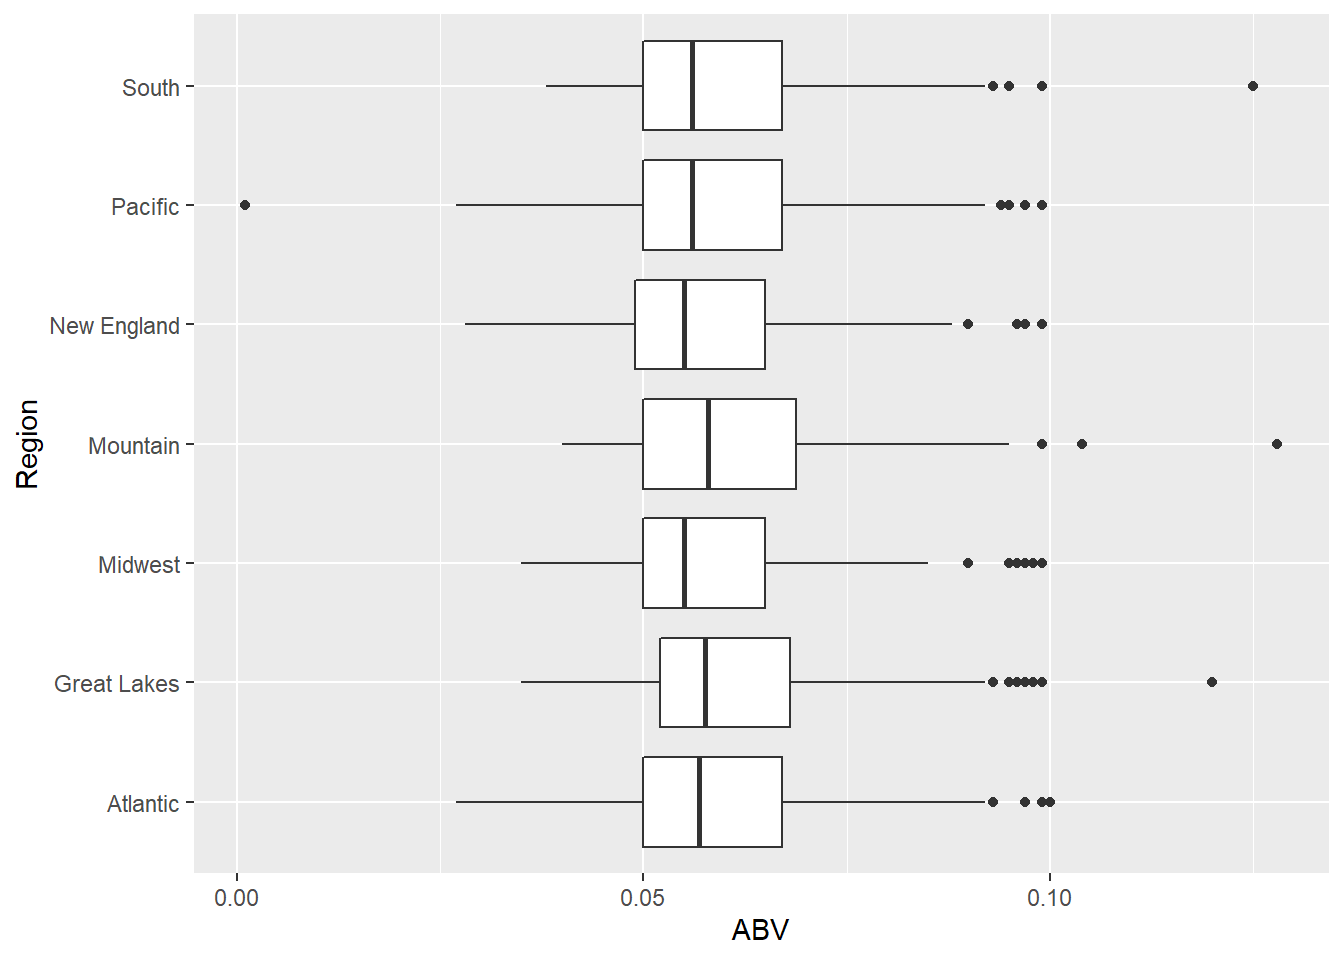
\includegraphics{Case_Study_01_files/figure-latex/unnamed-chunk-10-1.pdf}

\begin{Shaded}
\begin{Highlighting}[]
\FunctionTok{ggplot}\NormalTok{(df, }\FunctionTok{aes}\NormalTok{(}\AttributeTok{x=}\NormalTok{ABV)) }\SpecialCharTok{+} \FunctionTok{geom\_histogram}\NormalTok{() }\SpecialCharTok{+} \FunctionTok{facet\_wrap}\NormalTok{(}\SpecialCharTok{\textasciitilde{}}\NormalTok{Region)}
\end{Highlighting}
\end{Shaded}

\begin{verbatim}
## `stat_bin()` using `bins = 30`. Pick better value with `binwidth`.
\end{verbatim}

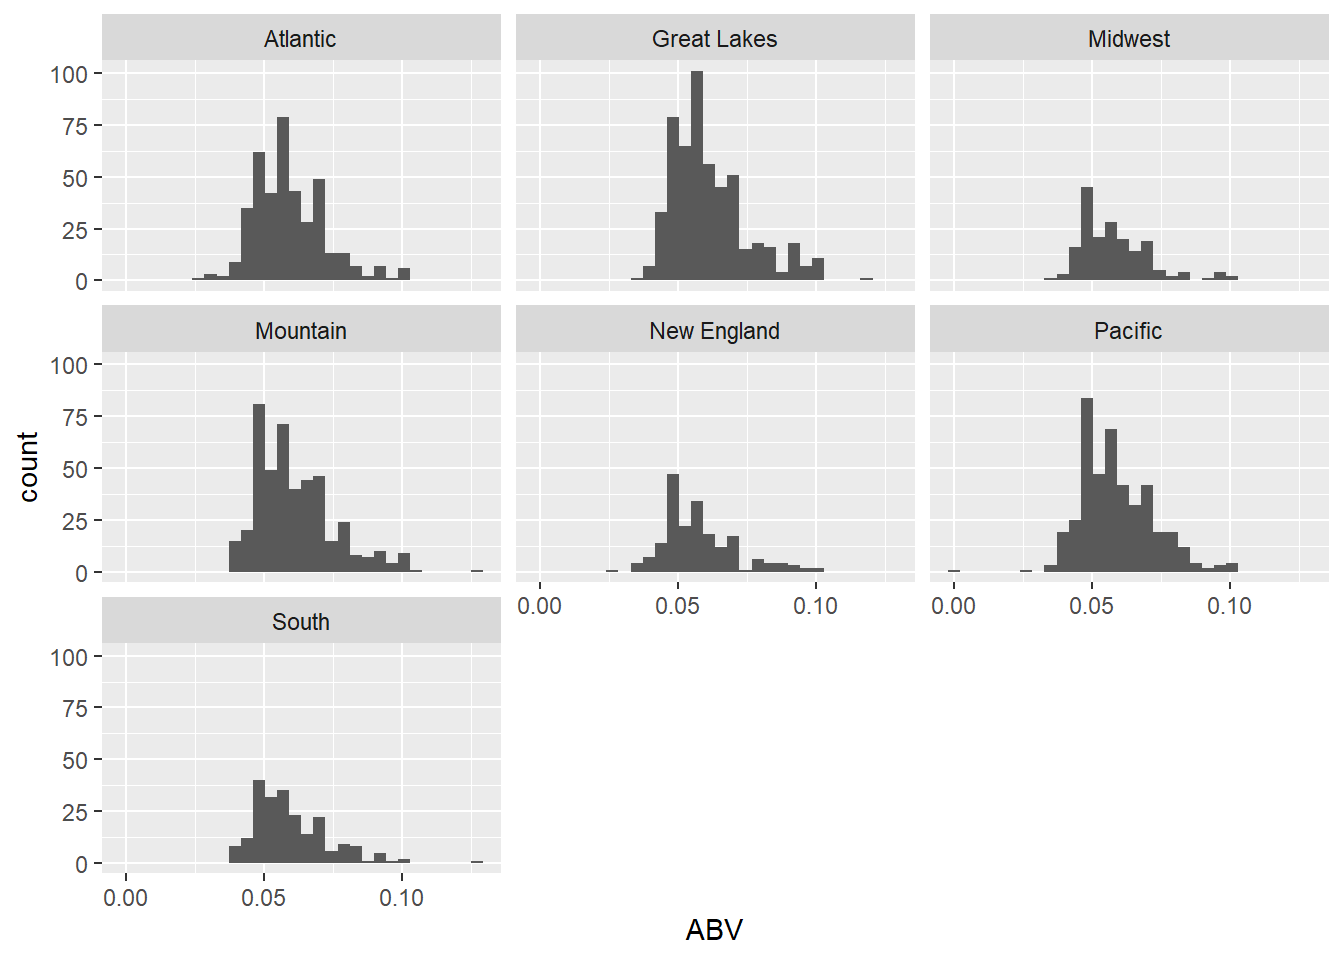
\includegraphics{Case_Study_01_files/figure-latex/unnamed-chunk-10-2.pdf}

\begin{Shaded}
\begin{Highlighting}[]
\CommentTok{\# IBU}
\FunctionTok{ggplot}\NormalTok{(df, }\FunctionTok{aes}\NormalTok{(}\AttributeTok{x=}\NormalTok{IBU, }\AttributeTok{y=}\NormalTok{Region)) }\SpecialCharTok{+} \FunctionTok{geom\_boxplot}\NormalTok{()}
\end{Highlighting}
\end{Shaded}

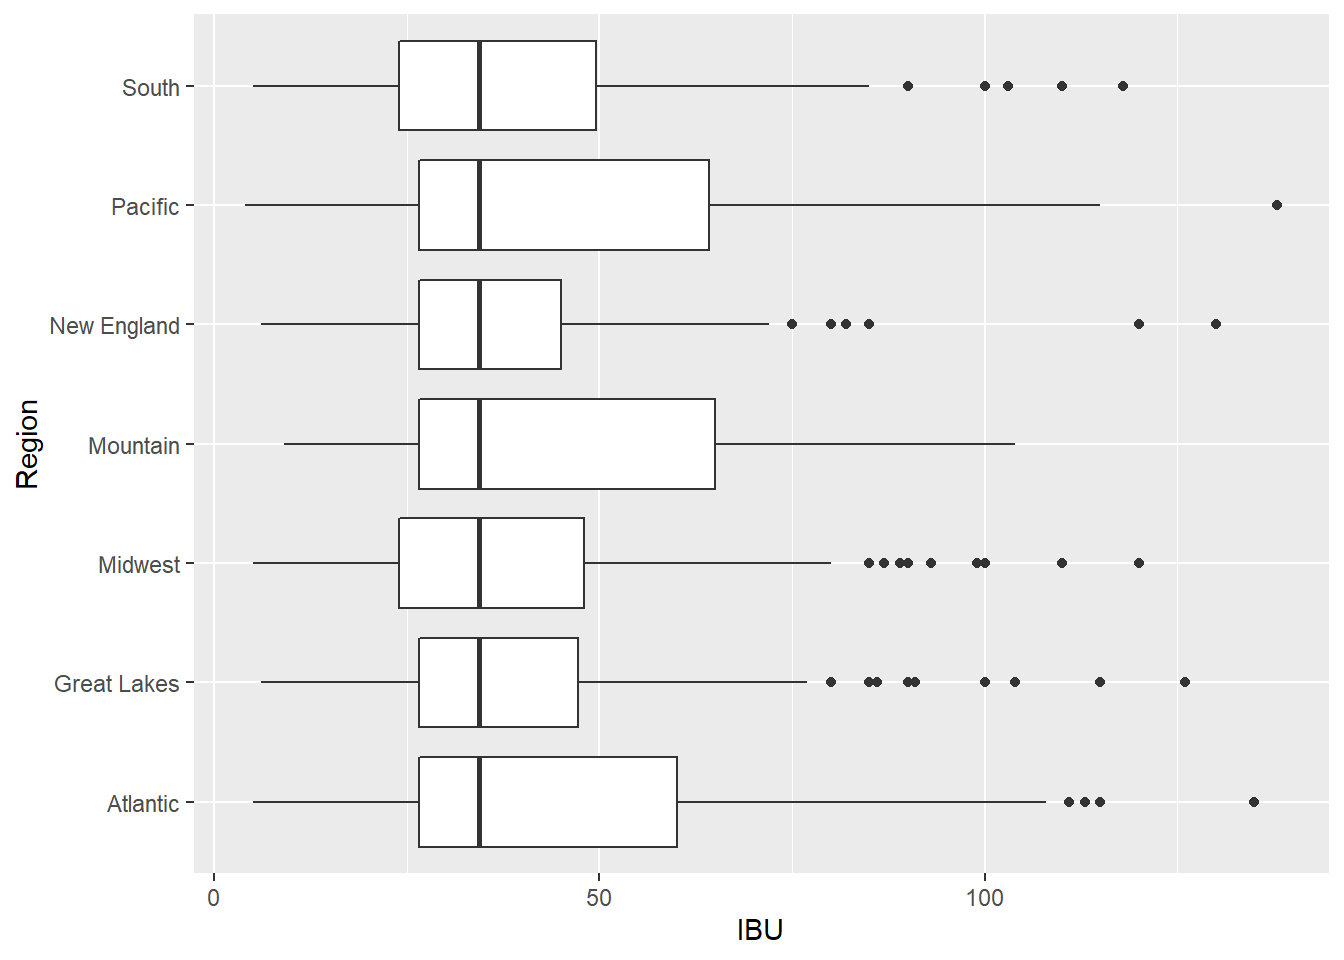
\includegraphics{Case_Study_01_files/figure-latex/unnamed-chunk-10-3.pdf}

\begin{Shaded}
\begin{Highlighting}[]
\FunctionTok{ggplot}\NormalTok{(df, }\FunctionTok{aes}\NormalTok{(}\AttributeTok{x=}\NormalTok{IBU)) }\SpecialCharTok{+} \FunctionTok{geom\_histogram}\NormalTok{() }\SpecialCharTok{+} \FunctionTok{facet\_wrap}\NormalTok{(}\SpecialCharTok{\textasciitilde{}}\NormalTok{Region)}
\end{Highlighting}
\end{Shaded}

\begin{verbatim}
## `stat_bin()` using `bins = 30`. Pick better value with `binwidth`.
\end{verbatim}

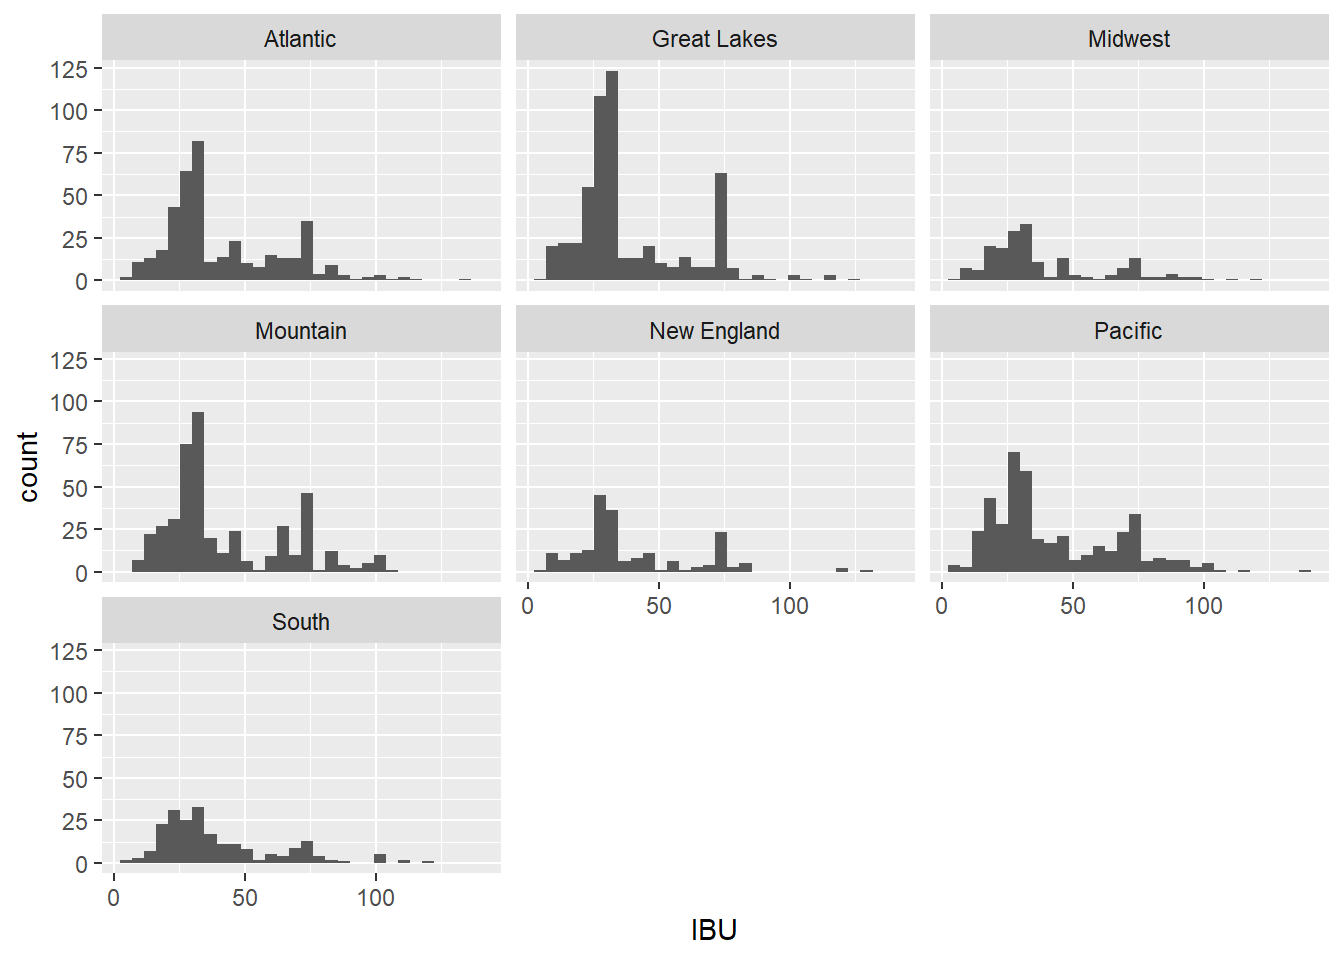
\includegraphics{Case_Study_01_files/figure-latex/unnamed-chunk-10-4.pdf}

\begin{Shaded}
\begin{Highlighting}[]
\CommentTok{\# We are assuming independence both with{-}in and between groups.}
\end{Highlighting}
\end{Shaded}

ABV: While regions have similar variances, I can't say that they are
normally distributed. Although the CLT may allows us to bypass this
assumption, I will stick with a non-parametric test to be safe.

IBU: There is overwhelming evidence that the distributions are not
normal and that regions do not have similar variance. Because of this, a
non-parametric test is required.

\hypertarget{kruskal-wallis-test}{%
\subsubsection{Kruskal Wallis Test}\label{kruskal-wallis-test}}

\begin{Shaded}
\begin{Highlighting}[]
\FunctionTok{kruskal.test}\NormalTok{(ABV}\SpecialCharTok{\textasciitilde{}}\NormalTok{Region, df)}
\end{Highlighting}
\end{Shaded}

\begin{verbatim}
## 
##  Kruskal-Wallis rank sum test
## 
## data:  ABV by Region
## Kruskal-Wallis chi-squared = 24.969, df = 6, p-value = 0.000346
\end{verbatim}

\begin{Shaded}
\begin{Highlighting}[]
\CommentTok{\# P{-}value \textless{} .05, so we say that there is evidence to suggest that at least one of the Region median ABVs is significantly different from the others.}

\FunctionTok{kruskal.test}\NormalTok{(IBU}\SpecialCharTok{\textasciitilde{}}\NormalTok{Region, df)}
\end{Highlighting}
\end{Shaded}

\begin{verbatim}
## 
##  Kruskal-Wallis rank sum test
## 
## data:  IBU by Region
## Kruskal-Wallis chi-squared = 11.366, df = 6, p-value = 0.07772
\end{verbatim}

\begin{Shaded}
\begin{Highlighting}[]
\CommentTok{\# P{-}value \textgreater{} .05, so we say that there is not enough evidence to suggest that there is a difference in Region{-}specific ABV medians.}
\end{Highlighting}
\end{Shaded}

The Kruskal-Wallis test provides sufficient evidence to suggest that at
least one region has a mean ABV that differs significantly from the
others. Further testing down below (P-value = .00035).

The Kruskal-Wallis test suggests that there is not enough evidence to
say that any region's mean IBU differs significantly from any others. No
further testing needed (P-value = .0778).

\hypertarget{to-find-which-exact-regions-have-differing-median-abvs-we-will-use-rank-sum-tests.-the-function-below-calculates-all-combinations-of-the-regions-in-our-df-and-tests-them-using-wilcox.test.}{%
\subsubsection{To find which exact regions have differing median ABVs,
we will use Rank Sum Tests. The function below calculates all
combinations of the regions in our df and tests them using
wilcox.test.}\label{to-find-which-exact-regions-have-differing-median-abvs-we-will-use-rank-sum-tests.-the-function-below-calculates-all-combinations-of-the-regions-in-our-df-and-tests-them-using-wilcox.test.}}

\begin{Shaded}
\begin{Highlighting}[]
\NormalTok{regions }\OtherTok{\textless{}{-}} \FunctionTok{unique}\NormalTok{(}\FunctionTok{as.character}\NormalTok{(df}\SpecialCharTok{$}\NormalTok{Region))}
\CommentTok{\# Pull regions into a list}

\NormalTok{wilcoxon\_tester }\OtherTok{\textless{}{-}} \ControlFlowTok{function}\NormalTok{(myVar) \{}
\NormalTok{  region\_x }\OtherTok{\textless{}{-}} \FunctionTok{character}\NormalTok{()}
\NormalTok{  region\_y }\OtherTok{\textless{}{-}} \FunctionTok{character}\NormalTok{()}
\NormalTok{  p\_value }\OtherTok{\textless{}{-}} \FunctionTok{numeric}\NormalTok{()}
  
  \ControlFlowTok{for}\NormalTok{ (i }\ControlFlowTok{in} \DecValTok{1}\SpecialCharTok{:}\FunctionTok{length}\NormalTok{(regions)) \{}
    
    \ControlFlowTok{for}\NormalTok{ (j }\ControlFlowTok{in} \DecValTok{1}\SpecialCharTok{:}\FunctionTok{length}\NormalTok{(regions)) \{}
      
      \ControlFlowTok{if}\NormalTok{ (j }\SpecialCharTok{!=}\NormalTok{ i) \{}
\NormalTok{        j\_df }\OtherTok{\textless{}{-}}\NormalTok{ df }\SpecialCharTok{\%\textgreater{}\%} \FunctionTok{filter}\NormalTok{(Region }\SpecialCharTok{==}\NormalTok{ regions[j]) }\SpecialCharTok{\%\textgreater{}\%} \FunctionTok{pull}\NormalTok{(\{\{myVar\}\})}
\NormalTok{        i\_df }\OtherTok{\textless{}{-}}\NormalTok{ df }\SpecialCharTok{\%\textgreater{}\%} \FunctionTok{filter}\NormalTok{(Region }\SpecialCharTok{==}\NormalTok{ regions[i]) }\SpecialCharTok{\%\textgreater{}\%} \FunctionTok{pull}\NormalTok{(\{\{myVar\}\})}
\NormalTok{        test }\OtherTok{\textless{}{-}} \FunctionTok{wilcox.test}\NormalTok{(}\AttributeTok{x=}\NormalTok{j\_df, }\AttributeTok{y=}\NormalTok{i\_df, }\AttributeTok{alternative=}\StringTok{\textquotesingle{}two.sided\textquotesingle{}}\NormalTok{)}
        
        \ControlFlowTok{if}\NormalTok{ (test}\SpecialCharTok{$}\NormalTok{p.value }\SpecialCharTok{\textless{}}\NormalTok{ .}\DecValTok{05}\NormalTok{) \{}
\NormalTok{          region\_x }\OtherTok{\textless{}{-}} \FunctionTok{append}\NormalTok{(region\_x, regions[i])}
\NormalTok{          region\_y }\OtherTok{\textless{}{-}} \FunctionTok{append}\NormalTok{(region\_y, regions[j])}
\NormalTok{          p\_value }\OtherTok{\textless{}{-}} \FunctionTok{append}\NormalTok{(p\_value, }\FunctionTok{round}\NormalTok{(test}\SpecialCharTok{$}\NormalTok{p.value, }\DecValTok{4}\NormalTok{))}
\NormalTok{        \}}
\NormalTok{      \}}
\NormalTok{    \}}
\NormalTok{  \}}
\NormalTok{  wilcox\_results }\OtherTok{\textless{}{-}} \FunctionTok{data.frame}\NormalTok{(}\StringTok{\textquotesingle{}Region\_x\textquotesingle{}}\OtherTok{=}\NormalTok{region\_x, }\StringTok{\textquotesingle{}Region\_y\textquotesingle{}}\OtherTok{=}\NormalTok{region\_y, }\StringTok{\textquotesingle{}P\_value\textquotesingle{}}\OtherTok{=}\NormalTok{p\_value)}
\NormalTok{\}}

\CommentTok{\# Testing....will print out all tests that are significant.}
\NormalTok{wilcox\_results }\OtherTok{\textless{}{-}} \FunctionTok{wilcoxon\_tester}\NormalTok{(ABV)}

\CommentTok{\# Filters out all even rows (each test result is duplicated)}
\NormalTok{wilcox\_results }\OtherTok{\textless{}{-}}\NormalTok{ wilcox\_results }\SpecialCharTok{\%\textgreater{}\%} \FunctionTok{arrange}\NormalTok{(P\_value)}
\NormalTok{wilcox\_results}\SpecialCharTok{$}\NormalTok{odd }\OtherTok{\textless{}{-}} \FunctionTok{seq\_len}\NormalTok{(}\FunctionTok{nrow}\NormalTok{(wilcox\_results)) }\SpecialCharTok{\%\%} \DecValTok{2}

\NormalTok{wilcox\_results }\SpecialCharTok{\%\textgreater{}\%} \FunctionTok{arrange}\NormalTok{(Region\_x) }\SpecialCharTok{\%\textgreater{}\%} \FunctionTok{filter}\NormalTok{(odd }\SpecialCharTok{==} \DecValTok{1}\NormalTok{)}
\end{Highlighting}
\end{Shaded}

\begin{verbatim}
##      Region_x    Region_y P_value odd
## 1    Atlantic Great Lakes  0.0409   1
## 2     Midwest Great Lakes  0.0024   1
## 3    Mountain New England  0.0004   1
## 4    Mountain     Midwest  0.0055   1
## 5 New England Great Lakes  0.0001   1
## 6 New England    Atlantic  0.0310   1
## 7     Pacific Great Lakes  0.0144   1
## 8     Pacific    Mountain  0.0259   1
\end{verbatim}

The Rank Sum Tests above tell us that 8 out of the 21 region
combinations have significantly different mean ABVs. Displayed along the
two regions is the p-value from the associated test.

Interesting Notes: A. The `South' region does not appear. Therefore, it
is similar to all other regions. B. The `Great Lakes' region appears 4
times, making it the most unique region.

\hypertarget{conclusion}{%
\section{Conclusion:}\label{conclusion}}

In conclusion, we found that the breweries in the US are mostly located
in high density states like Texas and California. We saw that the median
beer ABV does not vary that much between states, and the ABV
distribution shows a tail of more alcoholic beers towards the higher end
of the ABV spectrum. This observation is consistent with the idea that
craft beers are becoming more and more popular in the US. We also saw a
moderate positive correlation between ABV and IBU. Our hypothesis is
that this correlation exists because adding hops, a key ingredient in
most beers, will make a beer more alcoholic and more bitter. Although
the craft beer trend is rising, Budweiser would likely benefit from a
lower ABV beer, possibly because most people do not enjoy the
bitterness. To further analyze the correlation between ABV and IBU,
particularly in Ales vs IPA's, we ran the data through a KNN model. The
model came to show that, given a beer's ABV and IBU, we could predict
whether that beer was an Ale or IPA with an accuracy of over 91\%! We
also had very similar accuracy results when using a Naïve-Bayes model.
In both cases, the models showed that ABV and IBU do not significantly
vary in beer styles. Finally, our statistical tests (Kruskal-Wallis \&
Rank Sum) highlights which regions had significantly different mean ABVs
or IBUs. Using the feedback from these tests, Budweiser can consider how
the ABV of a new product would fit into each region's existing range of
beers.

\end{document}
